\UseRawInputEncoding
%DIF LATEXDIFF DIFFERENCE FILE
%DIF DEL ./old/compiled_v077.tex   Sun Jan 14 22:51:18 2024
%DIF ADD ./compiled.tex            Sun Jan 14 23:23:45 2024

%%%%%%%%%%%%%%%%%%%%%%%%%%%%%%%%%%%%%%%%%%%%%%%%%%%%%%%%%%%%%%%%%%%%%%%%%%%%%%%%
%% SETTINGS
%%%%%%%%%%%%%%%%%%%%%%%%%%%%%%%%%%%%%%%%%%%%%%%%%%%%%%%%%%%%%%%%%%%%%%%%%%%%%%%%
%% Columns
\documentclass[final,3p,times,twocolumn]{elsarticle}
%% Use the options 1p,twocolumn; 3p; 3p,twocolumn; 5p; or 5p,twocolumn
%% for a journal layout:
%% \documentclass[final,1p,times]{elsarticle}
%% \documentclass[final,1p,times,twocolumn]{elsarticle}
%% \documentclass[final,3p,times]{elsarticle}
%% \documentclass[final,3p,times,twocolumn]{elsarticle}
%% \documentclass[final,5p,times]{elsarticle}
%% \documentclass[final,5p,times,twocolumn]{elsarticle}
%% \documentclass[preprint,review,12pt]{elsarticle}

%% Image width
\newlength{\imagewidth}
\newlength{\imagescale}
%% preamble
\usepackage[english]{babel}
\usepackage[table]{xcolor} % For coloring tables
\usepackage{booktabs} % For professional quality tables
\usepackage{colortbl} % For coloring cells in tables
\usepackage{amsmath, amssymb} % For mathematical symbols and environments
\usepackage{amsthm} % For theorem-like environments
\usepackage{lipsum} % just for sample text
\usepackage{natbib}
\usepackage{graphicx}
\usepackage{indentfirst}
\usepackage{bashful}
\usepackage[margin=10pt,font=small,labelfont=bf,labelsep=endash]{caption}
\usepackage{graphicx}
\usepackage{calc}
\usepackage[T1]{fontenc} % [REVISED]
\usepackage[utf8]{inputenc} % [REVISED]
\usepackage{hyperref}
\usepackage{accsupp}
%% Line numbers
\linespread{1.1}
% \linenumbers
% Tables
\usepackage[pass]{geometry}
\usepackage{pdflscape}
\usepackage{csvsimple}
\usepackage{xltabular}
\usepackage{booktabs}
\usepackage{siunitx}
\usepackage{makecell}
\sisetup{round-mode=figures,round-precision=3}
\renewcommand\theadfont{\bfseries}
\renewcommand\theadalign{c}
\newcolumntype{C}[1]{>{\centering\arraybackslash}m{#1}}
\renewcommand{\arraystretch}{1.5}
\definecolor{lightgray}{gray}{0.95}

%% Diff
\usepackage{xcolor}
% Define commands for highlighting
% diff
\usepackage[most]{tcolorbox} % for boxes with transparency
% Define colors with transparency (opacity value)
\definecolor{GreenBG}{rgb}{0,1,0}
\definecolor{RedBG}{rgb}{1,0,0}
% Define tcolorbox environments for highlighting
\newtcbox{\greenhighlight}[1][]{%
  on line,
  colframe=GreenBG,
  colback=GreenBG!50!white, % 50% transparent green
  boxrule=0pt,
  arc=0pt,
  boxsep=0pt,
  left=1pt,
  right=1pt,
  top=2pt,
  bottom=2pt,
  tcbox raise base
}
\newtcbox{\redhighlight}[1][]{%
  on line,
  colframe=RedBG,
  colback=RedBG!50!white, % 50% transparent red
  boxrule=0pt,
  arc=0pt,
  boxsep=0pt,
  left=1pt,
  right=1pt,
  top=2pt,
  bottom=2pt,
  tcbox raise base
}
\newcommand{\REDSTARTS}{\color{red}}
\newcommand{\REDENDS}{\color{black}}
\newcommand{\GREENSTARTS}{\color{green}}
\newcommand{\GREENENDS}{\color{black}}

% New command to read word counts
\newread\wordcount
\newcommand\readwordcount[1]{%
  \openin\wordcount=#1
  \read\wordcount to \thewordcount
  \closein\wordcount
  \thewordcount
}

%%%%%%%%%%%%%%%%%%%%%%%%%%%%%%%%%%%%%%%%%%%%%%%%%%%%%%%%%%%%%%%%%%%%%%%%%%%%%%%%
%% JOURNAL NAME
%%%%%%%%%%%%%%%%%%%%%%%%%%%%%%%%%%%%%%%%%%%%%%%%%%%%%%%%%%%%%%%%%%%%%%%%%%%%%%%%
\journal{Heliyon}
%%%%%%%%%%%%%%%%%%%%%%%%%%%%%%%%%%%%%%%%%%%%%%%%%%%%%%%%%%%%%%%%%%%%%%%%%%%%%%%%
%% DOCUMENT STARTS
%%%%%%%%%%%%%%%%%%%%%%%%%%%%%%%%%%%%%%%%%%%%%%%%%%%%%%%%%%%%%%%%%%%%%%%%%%%%%%%%
%DIF PREAMBLE EXTENSION ADDED BY LATEXDIFF
%DIF UNDERLINE PREAMBLE %DIF PREAMBLE
\RequirePackage[normalem]{ulem} %DIF PREAMBLE
\RequirePackage{color}\definecolor{RED}{rgb}{1,0,0}\definecolor{BLUE}{rgb}{0,0,1} %DIF PREAMBLE
\providecommand{\DIFaddtex}[1]{{\protect\color{blue}\uwave{#1}}} %DIF PREAMBLE
\providecommand{\DIFdeltex}[1]{{\protect\color{red}\sout{#1}}}                      %DIF PREAMBLE
%DIF SAFE PREAMBLE %DIF PREAMBLE
\providecommand{\DIFaddbegin}{} %DIF PREAMBLE
\providecommand{\DIFaddend}{} %DIF PREAMBLE
\providecommand{\DIFdelbegin}{} %DIF PREAMBLE
\providecommand{\DIFdelend}{} %DIF PREAMBLE
\providecommand{\DIFmodbegin}{} %DIF PREAMBLE
\providecommand{\DIFmodend}{} %DIF PREAMBLE
%DIF FLOATSAFE PREAMBLE %DIF PREAMBLE
\providecommand{\DIFaddFL}[1]{\DIFadd{#1}} %DIF PREAMBLE
\providecommand{\DIFdelFL}[1]{\DIFdel{#1}} %DIF PREAMBLE
\providecommand{\DIFaddbeginFL}{} %DIF PREAMBLE
\providecommand{\DIFaddendFL}{} %DIF PREAMBLE
\providecommand{\DIFdelbeginFL}{} %DIF PREAMBLE
\providecommand{\DIFdelendFL}{} %DIF PREAMBLE
%DIF HYPERREF PREAMBLE %DIF PREAMBLE
\providecommand{\DIFadd}[1]{\texorpdfstring{\DIFaddtex{#1}}{#1}} %DIF PREAMBLE
\providecommand{\DIFdel}[1]{\texorpdfstring{\DIFdeltex{#1}}{}} %DIF PREAMBLE
\newcommand{\DIFscaledelfig}{0.5}
%DIF HIGHLIGHTGRAPHICS PREAMBLE %DIF PREAMBLE
\RequirePackage{settobox} %DIF PREAMBLE
\RequirePackage{letltxmacro} %DIF PREAMBLE
\newsavebox{\DIFdelgraphicsbox} %DIF PREAMBLE
\newlength{\DIFdelgraphicswidth} %DIF PREAMBLE
\newlength{\DIFdelgraphicsheight} %DIF PREAMBLE
% store original definition of \includegraphics %DIF PREAMBLE
\LetLtxMacro{\DIFOincludegraphics}{\includegraphics} %DIF PREAMBLE
\newcommand{\DIFaddincludegraphics}[2][]{{\color{blue}\fbox{\DIFOincludegraphics[#1]{#2}}}} %DIF PREAMBLE
\newcommand{\DIFdelincludegraphics}[2][]{% %DIF PREAMBLE
\sbox{\DIFdelgraphicsbox}{\DIFOincludegraphics[#1]{#2}}% %DIF PREAMBLE
\settoboxwidth{\DIFdelgraphicswidth}{\DIFdelgraphicsbox} %DIF PREAMBLE
\settoboxtotalheight{\DIFdelgraphicsheight}{\DIFdelgraphicsbox} %DIF PREAMBLE
\scalebox{\DIFscaledelfig}{% %DIF PREAMBLE
\parbox[b]{\DIFdelgraphicswidth}{\usebox{\DIFdelgraphicsbox}\\[-\baselineskip] \rule{\DIFdelgraphicswidth}{0em}}\llap{\resizebox{\DIFdelgraphicswidth}{\DIFdelgraphicsheight}{% %DIF PREAMBLE
\setlength{\unitlength}{\DIFdelgraphicswidth}% %DIF PREAMBLE
\begin{picture}(1,1)% %DIF PREAMBLE
\thicklines\linethickness{2pt} %DIF PREAMBLE
{\color[rgb]{1,0,0}\put(0,0){\framebox(1,1){}}}% %DIF PREAMBLE
{\color[rgb]{1,0,0}\put(0,0){\line( 1,1){1}}}% %DIF PREAMBLE
{\color[rgb]{1,0,0}\put(0,1){\line(1,-1){1}}}% %DIF PREAMBLE
\end{picture}% %DIF PREAMBLE
}\hspace*{3pt}}} %DIF PREAMBLE
} %DIF PREAMBLE
\LetLtxMacro{\DIFOaddbegin}{\DIFaddbegin} %DIF PREAMBLE
\LetLtxMacro{\DIFOaddend}{\DIFaddend} %DIF PREAMBLE
\LetLtxMacro{\DIFOdelbegin}{\DIFdelbegin} %DIF PREAMBLE
\LetLtxMacro{\DIFOdelend}{\DIFdelend} %DIF PREAMBLE
\DeclareRobustCommand{\DIFaddbegin}{\DIFOaddbegin \let\includegraphics\DIFaddincludegraphics} %DIF PREAMBLE
\DeclareRobustCommand{\DIFaddend}{\DIFOaddend \let\includegraphics\DIFOincludegraphics} %DIF PREAMBLE
\DeclareRobustCommand{\DIFdelbegin}{\DIFOdelbegin \let\includegraphics\DIFdelincludegraphics} %DIF PREAMBLE
\DeclareRobustCommand{\DIFdelend}{\DIFOaddend \let\includegraphics\DIFOincludegraphics} %DIF PREAMBLE
\LetLtxMacro{\DIFOaddbeginFL}{\DIFaddbeginFL} %DIF PREAMBLE
\LetLtxMacro{\DIFOaddendFL}{\DIFaddendFL} %DIF PREAMBLE
\LetLtxMacro{\DIFOdelbeginFL}{\DIFdelbeginFL} %DIF PREAMBLE
\LetLtxMacro{\DIFOdelendFL}{\DIFdelendFL} %DIF PREAMBLE
\DeclareRobustCommand{\DIFaddbeginFL}{\DIFOaddbeginFL \let\includegraphics\DIFaddincludegraphics} %DIF PREAMBLE
\DeclareRobustCommand{\DIFaddendFL}{\DIFOaddendFL \let\includegraphics\DIFOincludegraphics} %DIF PREAMBLE
\DeclareRobustCommand{\DIFdelbeginFL}{\DIFOdelbeginFL \let\includegraphics\DIFdelincludegraphics} %DIF PREAMBLE
\DeclareRobustCommand{\DIFdelendFL}{\DIFOaddendFL \let\includegraphics\DIFOincludegraphics} %DIF PREAMBLE
%DIF LISTINGS PREAMBLE %DIF PREAMBLE
\RequirePackage{listings} %DIF PREAMBLE
\RequirePackage{color} %DIF PREAMBLE
\lstdefinelanguage{DIFcode}{ %DIF PREAMBLE
%DIF DIFCODE_UNDERLINE %DIF PREAMBLE
  moredelim=[il][\color{red}\sout]{\%DIF\ <\ }, %DIF PREAMBLE
  moredelim=[il][\color{blue}\uwave]{\%DIF\ >\ } %DIF PREAMBLE
} %DIF PREAMBLE
\lstdefinestyle{DIFverbatimstyle}{ %DIF PREAMBLE
	language=DIFcode, %DIF PREAMBLE
	basicstyle=\ttfamily, %DIF PREAMBLE
	columns=fullflexible, %DIF PREAMBLE
	keepspaces=true %DIF PREAMBLE
} %DIF PREAMBLE
\lstnewenvironment{DIFverbatim}{\lstset{style=DIFverbatimstyle}}{} %DIF PREAMBLE
\lstnewenvironment{DIFverbatim*}{\lstset{style=DIFverbatimstyle,showspaces=true}}{} %DIF PREAMBLE
%DIF END PREAMBLE EXTENSION ADDED BY LATEXDIFF

\begin{document}

%%%%%%%%%%%%%%%%%%%%%%%%%%%%%%%%%%%%%%%%%%%%%%%%%%%%%%%%%%%%%%%%%%%%%%%%%%%%%%%%
%% Frontmatter
%%%%%%%%%%%%%%%%%%%%%%%%%%%%%%%%%%%%%%%%%%%%%%%%%%%%%%%%%%%%%%%%%%%%%%%%%%%%%%%%
\begin{frontmatter}
\begin{highlights}
\pdfbookmark[1]{Highlights}{highlights}

\item Neural trajectories in the hippocampus exhibited greater variability during a working memory (WM) task compared to those in the entorhinal cortex and amygdala regions.

\item The distance of neural trajectories between encoding and retrieval states in the hippocampus was memory-load dependent during a WM task.


\item Hippocampal neural trajectories fluctuated between the encoding and retrieval states in a task-dependent manner during both baseline and sharp-wave ripple (SWR) periods.

\item Hippocampal neural trajectories shifted from encoding to retrieval states during SWR period.

\end{highlights}\title{
Hippocampal Neural Fluctuations Between Memory Encoding and Retrieval States During a Working Memory Task in Humans
}\author[1]{Yusuke Watanabe\corref{cor1}}
\author[2,3,4]{Yuji Ikegaya}
\author[1,5]{Takufumi Yanagisawa}

\address[1]{Institute for Advanced Cocreation studies, Osaka University, 2-2 Yamadaoka, Suita, 565-0871, Osaka, Japan}
\address[2]{Graduate School of Pharmaceutical Sciences, The University of Tokyo, 7-3-1 Hongo, Tokyo, 113-0033, Japan}
\address[3]{Institute for AI and Beyond, The University of Tokyo, 7-3-1 Hongo, Tokyo, 113-0033, Japan}
\address[4]{Center for Information and Neural Networks, National Institute of Information and Communications Technology, 1-4 Yamadaoka, Suita City, 565-0871, Osaka, Japan}
\address[5]{Department of Neurosurgery, Osaka University Graduate School of Medicine, 2-2 Yamadaoka, Osaka, 565-0871, Japan}

\cortext[cor1]{Corresponding author. Tel: +81-6-6879-3652 Email: ywatanabe@alumni.u-tokyo.ac.jp}

%%Graphical abstract
%\pdfbookmark[1]{Graphical Abstract}{graphicalabstract}        
%\begin{graphicalabstract}
%\includegraphics{grabs}
%\end{graphicalabstract}
\begin{abstract}
\pdfbookmark[1]{Abstract}{abstract}
Working memory (WM) is \DIFdelbegin \DIFdel{crucial for numerous }\DIFdelend \DIFaddbegin \DIFadd{vital for many }\DIFaddend cognitive functions, \DIFdelbegin \DIFdel{but }\DIFdelend \DIFaddbegin \DIFadd{although }\DIFaddend the neural mechanisms \DIFdelbegin \DIFdel{that underpin }\DIFdelend \DIFaddbegin \DIFadd{underlying }\DIFaddend its operation are not \DIFdelbegin \DIFdel{fully comprehended. The hippocampus and its }\DIFdelend \DIFaddbegin \DIFadd{yet fully understood. Although the hippocampus and }\DIFaddend associated sharp-wave ripples (SWRs) --- brief, synchronized oscillations \DIFdelbegin \DIFdel{observed within }\DIFdelend \DIFaddbegin \DIFadd{within it }\DIFaddend --- have been \DIFdelbegin \DIFdel{studied due }\DIFdelend \DIFaddbegin \DIFadd{explored owing }\DIFaddend to their role in memory consolidation and retrieval, \DIFdelbegin \DIFdel{albeit, the full extent }\DIFdelend \DIFaddbegin \DIFadd{a comprehensive understanding }\DIFaddend of their involvement \DIFdelbegin \DIFdel{with }\DIFdelend \DIFaddbegin \DIFadd{in }\DIFaddend WM tasks is \DIFdelbegin \DIFdel{yet to be thoroughly explored}\DIFdelend \DIFaddbegin \DIFadd{pending further investigation}\DIFaddend . This study \DIFdelbegin \DIFdel{proves that }\DIFdelend \DIFaddbegin \DIFadd{reveals that a }\DIFaddend WM task introduces unique dynamics \DIFdelbegin \DIFdel{in }\DIFdelend \DIFaddbegin \DIFadd{into }\DIFaddend the multi-unit activity patterns of the hippocampus, \DIFdelbegin \DIFdel{particularly during SWR periods}\DIFdelend \DIFaddbegin \DIFadd{primarily during SWR episodes}\DIFaddend . We analyzed intracranial electroencephalography data \DIFdelbegin \DIFdel{, }\DIFdelend collected from the medial temporal lobe (MTL) of nine epilepsy patients \DIFdelbegin \DIFdel{during }\DIFdelend \DIFaddbegin \DIFadd{performing }\DIFaddend an eight-second Sternberg task. Using \DIFdelbegin \DIFdel{a }\DIFdelend Gaussian-process factor analysis, we extracted low-dimensional neural representations or neural trajectories (NT) within MTL regions throughout the Sternberg WM task. The analysis \DIFdelbegin \DIFdel{showed significant variances in the hippocampal NT when compared with that of }\DIFdelend \DIFaddbegin \DIFadd{demonstrated substantial differences in hippocampal NT compared to that in }\DIFaddend the entorhinal cortex and the amygdala. Additionally, the NT distance between the encoding and retrieval phases was \DIFdelbegin \DIFdel{found to be }\DIFdelend dependent on the memory load. \DIFdelbegin \DIFdel{Significantly, the hippocampal NT varied during the retrieval phase between }\DIFdelend \DIFaddbegin \DIFadd{Notably, hippocampal NT distinguished }\DIFaddend encoding and retrieval states \DIFaddbegin \DIFadd{during the retrieval phase }\DIFaddend in a task-dependent manner. These \DIFdelbegin \DIFdel{variations }\DIFdelend \DIFaddbegin \DIFadd{differences }\DIFaddend transitioned from encoding to retrieval states \DIFdelbegin \DIFdel{during }\DIFdelend \DIFaddbegin \DIFadd{in the presence of }\DIFaddend SWR episodes. These \DIFdelbegin \DIFdel{findings stress }\DIFdelend \DIFaddbegin \DIFadd{results emphasize }\DIFaddend the importance of the hippocampus in WM tasks \DIFdelbegin \DIFdel{, }\DIFdelend and propose a new \DIFdelbegin \DIFdel{hypothes that }\DIFdelend \DIFaddbegin \DIFadd{hypothesis: }\DIFaddend the hippocampus transitions its functional state from encoding to retrieval during SWRs in WM tasks.
\end{abstract}% \pdfbookmark[1]{Keywords}{keywords}                
\begin{keyword}
working memory \sep memory load \sep hippocampus \sep sharp-wave ripples \sep humans
\end{keyword}
\end{frontmatter}

%%%%%%%%%%%%%%%%%%%%%%%%%%%%%%%%%%%%%%%%%%%%%%%%%%%%%%%%%%%%%%%%%%%%%%%%%%%%%%%%
%% Counters
%%%%%%%%%%%%%%%%%%%%%%%%%%%%%%%%%%%%%%%%%%%%%%%%%%%%%%%%%%%%%%%%%%%%%%%%%%%%%%%%
\begin{wordcount*}
\readwordcount{./src/.figure_count.txt} figures, \readwordcount{./src/.table_count.txt} tables, \readwordcount{./src/.abstract_count.txt} words for abstract, and \readwordcount{./src/.imrd_count.txt} words for main text
\end{wordcount*}
%%%%%%%%%%%%%%%%%%%%%%%%%%%%%%%%%%%%%%%%%%%%%%%%%%%%%%%%%%%%%%%%%%%%%%%%%%%%%%%%
%% IMRaD
%%%%%%%%%%%%%%%%%%%%%%%%%%%%%%%%%%%%%%%%%%%%%%%%%%%%%%%%%%%%%%%%%%%%%%%%%%%%%%%%

%%%%%%%%%%%%%%%%%%%%%%%%%%%%%%%%%%%%%%%%%%%%%%%%%%%%%%%%%%%%%%%%%%%%%%%%%%%%%%%%
%% INTRODUCTION
%%%%%%%%%%%%%%%%%%%%%%%%%%%%%%%%%%%%%%%%%%%%%%%%%%%%%%%%%%%%%%%%%%%%%%%%%%%%%%%%
\section{Introduction}
Working memory (WM) \DIFdelbegin \DIFdel{is crucial in everyday life; however, }\DIFdelend \DIFaddbegin \DIFadd{plays an essential role in everyday activities, yet comprehensive understanding of }\DIFaddend its neural mechanism\DIFdelbegin \DIFdel{has yet to be fully elucidated. Specifically, }\DIFdelend \DIFaddbegin \DIFadd{, including }\DIFaddend the hippocampus's involvement in WM processing, \DIFdelbegin \DIFdel{a pivotal }\DIFdelend \DIFaddbegin \DIFadd{remains elusive. The hippocampus, a central }\DIFaddend region for memory, is the \DIFdelbegin \DIFdel{subject of ongoing }\DIFdelend \DIFaddbegin \DIFadd{focus of continuous }\DIFaddend research \cite{scoville_loss_1957} \cite{squire_legacy_2009}  \cite{boran_persistent_2019} \cite{kaminski_persistently_2017} \cite{kornblith_persistent_2017} \cite{faraut_dataset_2018} \cite{borders_hippocampus_2022} \cite{li_functional_2023} \cite{dimakopoulos_information_2022}. \DIFdelbegin \DIFdel{Understanding the hippocampus’ role }\DIFdelend \DIFaddbegin \DIFadd{Gaining insight into the role of the hippocampus }\DIFaddend in working memory is \DIFdelbegin \DIFdel{instrumental in deepening our comprehension }\DIFdelend \DIFaddbegin \DIFadd{key to enhancing our understanding }\DIFaddend of cognitive processes and could potentially \DIFdelbegin \DIFdel{enhance cognitive abilities}\DIFdelend \DIFaddbegin \DIFadd{improve cognitive capabilities}\DIFaddend .
\\
\indent
Current evidence suggests that \DIFdelbegin \DIFdel{a transient, synchronized oscillation, called }\DIFdelend sharp-wave ripples (SWRs)\DIFdelbegin \DIFdel{\mbox{%DIFAUXCMD
\cite{buzsaki_hippocampal_2015}}\hspace{0pt}%DIFAUXCMD
, is associated }\DIFdelend \DIFaddbegin \DIFadd{, a form of transient, synchronized oscillation, is linked }\DIFaddend with several cognitive functions. These \DIFaddbegin \DIFadd{functions }\DIFaddend include memory replay \cite{wilson_reactivation_1994} \cite{nadasdy_replay_1999} \cite{lee_memory_2002} \cite{diba_forward_2007} \cite{davidson_hippocampal_2009}, memory consolidation \cite{girardeau_selective_2009} \cite{ego-stengel_disruption_2010} \cite{fernandez-ruiz_long-duration_2019} \cite{kim_corticalhippocampal_2022}, memory recall \cite{wu_hippocampal_2017} \cite{norman_hippocampal_2019} \cite{norman_hippocampal_2021}, and neural plasticity \cite{behrens_induction_2005} \cite{norimoto_hippocampal_2018}. These \DIFdelbegin \DIFdel{associations }\DIFdelend \DIFaddbegin \DIFadd{ties }\DIFaddend suggest that SWR \DIFdelbegin \DIFdel{may be }\DIFdelend \DIFaddbegin \DIFadd{serve as }\DIFaddend a fundamental computational \DIFdelbegin \DIFdel{manifestation }\DIFdelend \DIFaddbegin \DIFadd{mechanism }\DIFaddend of hippocampal processing, contributing to \DIFdelbegin \DIFdel{working memory performance as well}\DIFdelend \DIFaddbegin \DIFadd{the performance of working memory}\DIFaddend .
\\
\indent
Recent studies \DIFdelbegin \DIFdel{have found }\DIFdelend \DIFaddbegin \DIFadd{show }\DIFaddend that low-dimensional representations in hippocampal neurons can \DIFdelbegin \DIFdel{explain WM task performances. Specifically}\DIFdelend \DIFaddbegin \DIFadd{account for WM task performance. In particular}\DIFaddend , the firing patterns of place cells \cite{okeefe_hippocampus_1971} \cite{okeefe_place_1976} \cite{ekstrom_cellular_2003} \cite{kjelstrup_finite_2008} \cite{harvey_intracellular_2009}, found in the hippocampus, \DIFdelbegin \DIFdel{have been identified }\DIFdelend \DIFaddbegin \DIFadd{were noted }\DIFaddend within dynamic, nonlinear three-dimensional hyperbolic spaces in rats \cite{zhang_hippocampal_2022}. \DIFdelbegin \DIFdel{Additionally}\DIFdelend \DIFaddbegin \DIFadd{Also}\DIFaddend , grid cells in the entorhinal cortex (EC)\DIFdelbegin \DIFdel{, which is the main pathway }\DIFdelend \DIFaddbegin \DIFadd{—the key conduit }\DIFaddend to the hippocampus \cite{naber_reciprocal_2001} \cite{van_strien_anatomy_2009} \cite{strange_functional_2014}\DIFdelbegin \DIFdel{, exhibited a }\DIFdelend \DIFaddbegin \DIFadd{—demonstrated }\DIFaddend toroidal geometry during exploration in rats \cite{gardner_toroidal_2022}.
\\
\indent
However, these studies primarily \DIFdelbegin \DIFdel{focus }\DIFdelend \DIFaddbegin \DIFadd{concentrate }\DIFaddend on spatial navigation in rodents \DIFdelbegin \DIFdel{, which poses limitations. To illustrate}\DIFdelend \DIFaddbegin \DIFadd{and consequently, feature limitations. For instance}\DIFaddend , the temporal resolution of navigation tasks is \DIFdelbegin \DIFdel{inadequate as }\DIFdelend \DIFaddbegin \DIFadd{insufficient because }\DIFaddend the timing of memory acquisition and recall \DIFdelbegin \DIFdel{is not clearly delineated. Consequently, there is a relative paucity of research on the impact }\DIFdelend \DIFaddbegin \DIFadd{has not been clearly defined. As a result, there are few studies examining the influence }\DIFaddend of SWRs on WM performance \cite{jadhav_awake_2012}. \DIFdelbegin \DIFdel{Further, the presence }\DIFdelend \DIFaddbegin \DIFadd{Furthermore, the existence }\DIFaddend of noise in signals recorded during rodent movement complicates the detection of SWRs \cite{Watanabe_2021}. \DIFdelbegin \DIFdel{Therefore, to clarify }\DIFdelend \DIFaddbegin \DIFadd{Hence, human research is needed to elucidate }\DIFaddend the relationship between SWRs and WM tasks\DIFdelbegin \DIFdel{, research with human subjects is necessary}\DIFdelend .
\\
\indent
\DIFdelbegin \DIFdel{Considering these factors }\DIFdelend \DIFaddbegin \DIFadd{Taking these factors into account}\DIFaddend , this study \DIFdelbegin \DIFdel{investigates }\DIFdelend \DIFaddbegin \DIFadd{explores }\DIFaddend the hypothesis that \DIFaddbegin \DIFadd{during SWR periods, }\DIFaddend hippocampal neurons exhibit \DIFdelbegin \DIFdel{unique }\DIFdelend \DIFaddbegin \DIFadd{distinct }\DIFaddend neural trajectories (NTs) in low-dimensional space \DIFdelbegin \DIFdel{, particularly during SWR periods, }\DIFdelend in response to WM tasks in humans. To \DIFdelbegin \DIFdel{test }\DIFdelend \DIFaddbegin \DIFadd{substantiate }\DIFaddend this hypothesis, we \DIFdelbegin \DIFdel{employed }\DIFdelend \DIFaddbegin \DIFadd{used }\DIFaddend a dataset of patients performing an eight-second Sternberg task (\DIFdelbegin \DIFdel{1 s }\DIFdelend \DIFaddbegin \DIFadd{one second }\DIFaddend for fixation, \DIFdelbegin \DIFdel{2 s }\DIFdelend \DIFaddbegin \DIFadd{two seconds }\DIFaddend for encoding, \DIFdelbegin \DIFdel{3 s }\DIFdelend \DIFaddbegin \DIFadd{three seconds }\DIFaddend for maintenance, and \DIFdelbegin \DIFdel{2 s }\DIFdelend \DIFaddbegin \DIFadd{two seconds }\DIFaddend for retrieval) with high temporal resolution. \DIFdelbegin \DIFdel{Intracranial }\DIFdelend \DIFaddbegin \DIFadd{For these patients, intracranial }\DIFaddend electroencephalography (iEEG) signals within the medial temporal lobe (MTL) were recorded \DIFdelbegin \DIFdel{for these patients }\DIFdelend \cite{boran_dataset_2020}. To investigate low-dimensional NTs, we \DIFdelbegin \DIFdel{utilized }\DIFdelend \DIFaddbegin \DIFadd{employed }\DIFaddend Gaussian-process factor analysis (GPFA), \DIFdelbegin \DIFdel{an established }\DIFdelend \DIFaddbegin \DIFadd{a proven }\DIFaddend method for analyzing neural population dynamics \cite{yu_gaussian-process_2009}.
\label{sec:introduction}
%%%%%%%%%%%%%%%%%%%%%%%%%%%%%%%%%%%%%%%%%%%%%%%%%%%%%%%%%%%%%%%%%%%%%%%%%%%%%%%%
%% METHODS
%%%%%%%%%%%%%%%%%%%%%%%%%%%%%%%%%%%%%%%%%%%%%%%%%%%%%%%%%%%%%%%%%%%%%%%%%%%%%%%%
\section{Methods}
\subsection{Dataset}
The \DIFdelbegin \DIFdel{dataset used in this study , which is publicly available , comprises nine epilepsy patients }\DIFdelend \DIFaddbegin \DIFadd{data for this study were obtained from a publicly available dataset involving nine patients with epilepsy }\DIFaddend performing a modified \DIFdelbegin \DIFdel{the }\DIFdelend Sternberg task \cite{boran_dataset_2020}. This task \DIFdelbegin \DIFdel{includes four phases}\DIFdelend \DIFaddbegin \DIFadd{encompasses four stages}\DIFaddend : fixation (1s), encoding (2s), maintenance (3s), and retrieval (2s). During the encoding phase, \DIFdelbegin \DIFdel{participants were presented with }\DIFdelend a set of four, six, or eight \DIFdelbegin \DIFdel{alphabet letters . They were then tasked with determining }\DIFdelend \DIFaddbegin \DIFadd{letters were presented to the participants. Subsequently, they were tasked with assessing }\DIFaddend whether a probe letter displayed during the retrieval phase \DIFdelbegin \DIFdel{had previously appeared (the }\DIFdelend \DIFaddbegin \DIFadd{was previously shown (indicating a }\DIFaddend correct response for \DIFaddbegin \DIFadd{the }\DIFaddend Match IN task) or not (\DIFdelbegin \DIFdel{the }\DIFdelend \DIFaddbegin \DIFadd{indicating a }\DIFaddend correct response for \DIFaddbegin \DIFadd{the }\DIFaddend Mismatch OUT task). Intracranial electroencephalography (iEEG) signals were \DIFdelbegin \DIFdel{captured with }\DIFdelend \DIFaddbegin \DIFadd{recorded at }\DIFaddend a 32 kHz sampling rate within a 0.5--5,000 Hz frequency range, \DIFdelbegin \DIFdel{using depth electrodes in the MTLregions: }\DIFdelend \DIFaddbegin \DIFadd{with depth electrodes placed in medial temporal lobe (MTL) regions including }\DIFaddend the anterior head \DIFaddbegin \DIFadd{and posterior body }\DIFaddend of the left and right hippocampus (AHL\DIFdelbegin \DIFdel{and AHR), the posterior body of the hippocampus (PHL}\DIFdelend \DIFaddbegin \DIFadd{, AHR, PHL, }\DIFaddend and PHR), the entorhinal cortex (ECL and ECR), and the amygdala (AL and AR), as \DIFdelbegin \DIFdel{depicted }\DIFdelend \DIFaddbegin \DIFadd{shown }\DIFaddend in Figure~\ref{fig:01}A and Table~\ref{tab:01}. The iEEG signals were \DIFdelbegin \DIFdel{subsequently }\DIFdelend \DIFaddbegin \DIFadd{then }\DIFaddend downsampled to 2 kHz. Correlations between variables such as set size and \DIFdelbegin \DIFdel{correct rate were examined }\DIFdelend \DIFaddbegin \DIFadd{accuracy rate were explored }\DIFaddend (Figure~\ref{fig:s01}S1). Multiunit spike \DIFdelbegin \DIFdel{timing was }\DIFdelend \DIFaddbegin \DIFadd{timings were }\DIFaddend determined via a spike sorting algorithm \cite{niediek_reliable_2016} using the Combinato package (\url{https://github.com/jniediek/combinato})(Figure~\ref{fig:01}C).

\subsection{Calculation of NT using GPFA}
\DIFdelbegin \DIFdel{NTs}\DIFdelend \DIFaddbegin \DIFadd{Neural trajectories (NTs)}\DIFaddend , also referred to as 'factors', in the hippocampus, EC, and amygdala were \DIFdelbegin \DIFdel{determined using GPFA }\DIFdelend \DIFaddbegin \DIFadd{identified using Gaussian-Process Factor Analysis (GPFA) }\DIFaddend \cite{yu_gaussian-process_2009} applied to \DIFdelbegin \DIFdel{the }\DIFdelend multi-unit activity data for each session, \DIFdelbegin \DIFdel{performed with the elephant }\DIFdelend \DIFaddbegin \DIFadd{using the Elephant }\DIFaddend package (\url{https://elephant.readthedocs.io/en/latest/reference/gpfa.html}). The bin size was set to 50 ms \DIFdelbegin \DIFdel{, without }\DIFdelend \DIFaddbegin \DIFadd{with no }\DIFaddend overlaps. Each factor was \DIFdelbegin \DIFdel{z-normalized }\DIFdelend \DIFaddbegin \DIFadd{Z-normalized }\DIFaddend across all sessions, and the Euclidean distance from the origin (\DIFdelbegin \DIFdel{$O$) was then }\DIFdelend \DIFaddbegin \DIFadd{O) was }\DIFaddend computed.
\\
\indent
For each NT \DIFdelbegin \DIFdel{within a region such as }\DIFdelend \DIFaddbegin \DIFadd{in respective regions like }\DIFaddend AHL, geometric medians ($\mathrm{g_{F}}$ for fixation, $\mathrm{g_{E}}$ for encoding, $\mathrm{g_{M}}$ for maintenance, and $\mathrm{g_{R}}$ for retrieval phase) were calculated by determining the \DIFdelbegin \DIFdel{median coordinates of the NT }\DIFdelend \DIFaddbegin \DIFadd{NT's median coordinates }\DIFaddend during the four phases. An optimal GPFA dimensionality was \DIFdelbegin \DIFdel{found to be }\DIFdelend \DIFaddbegin \DIFadd{identified as }\DIFaddend three using the elbow method \DIFdelbegin \DIFdel{obtained by examining }\DIFdelend \DIFaddbegin \DIFadd{drawn from investigating }\DIFaddend the log-likelihood values \DIFdelbegin \DIFdel{through }\DIFdelend \DIFaddbegin \DIFadd{via }\DIFaddend a three-fold cross-validation approach (Figure~\ref{fig:02}B).

\subsection{Identifying SWR candidates from hippocampal regions}
Potential \DIFdelbegin \DIFdel{SWR }\DIFdelend \DIFaddbegin \DIFadd{sharp wave-ripple (SWR) }\DIFaddend events within the hippocampus were \DIFdelbegin \DIFdel{detected }\DIFdelend \DIFaddbegin \DIFadd{identified }\DIFaddend using a widely \DIFdelbegin \DIFdel{used }\DIFdelend \DIFaddbegin \DIFadd{accepted }\DIFaddend method \cite{liu_consensus_2022}. \DIFdelbegin \DIFdel{LFP }\DIFdelend \DIFaddbegin \DIFadd{Local field potential (LFP) }\DIFaddend signals from a region of interest (ROI)\DIFdelbegin \DIFdel{like }\DIFdelend \DIFaddbegin \DIFadd{, such as }\DIFaddend AHL, were re-referenced by deducting the averaged signal from locations outside the ROI (\DIFdelbegin \DIFdel{for instance, }\DIFdelend \DIFaddbegin \DIFadd{including }\DIFaddend AHR, PHL, PHR, ECL, ECR, AL, and AR). The re-referenced LFP signals were then filtered \DIFdelbegin \DIFdel{with }\DIFdelend \DIFaddbegin \DIFadd{using }\DIFaddend a ripple-band filter (80--140 Hz) to \DIFdelbegin \DIFdel{determine }\DIFdelend \DIFaddbegin \DIFadd{identify }\DIFaddend SWR candidates, \DIFdelbegin \DIFdel{marked }\DIFdelend \DIFaddbegin \DIFadd{denoted }\DIFaddend as $\textrm{SWR}^+$ candidates. SWR detection \DIFdelbegin \DIFdel{was carried out using }\DIFdelend \DIFaddbegin \DIFadd{used }\DIFaddend a published tool (\url{https://github.com/Eden-Kramer-Lab/ripple_detection}) \cite{kay_hippocampal_2016}, with the bandpass range adjusted to 80--140 Hz for humans \DIFdelbegin \DIFdel{\mbox{%DIFAUXCMD
\cite{norman_hippocampal_2019} }\hspace{0pt}%DIFAUXCMD
\mbox{%DIFAUXCMD
\cite{norman_hippocampal_2021}}\hspace{0pt}%DIFAUXCMD
}\DIFdelend \DIFaddbegin \DIFadd{\mbox{%DIFAUXCMD
\cite{norman_hippocampal_2019, norman_hippocampal_2021}}\hspace{0pt}%DIFAUXCMD
}\DIFaddend , unlike the initial 150--250 Hz range typically applied to rodents.
\\
\indent
Control events for $\textrm{SWR}^+$ candidates, labeled as $\textrm{SWR}^-$ candidates, were \DIFdelbegin \DIFdel{detected }\DIFdelend \DIFaddbegin \DIFadd{discovered }\DIFaddend by randomly shuffling the timestamps of $\textrm{SWR}^+$ candidates across all trials and subjects. The resulting $\textrm{SWR}^+/\textrm{SWR}^-$ candidates were then visually inspected.

\subsection{Defining SWRs from \DIFdelbegin \DIFdel{putative }\DIFdelend \DIFaddbegin \DIFadd{potential }\DIFaddend hippocampal CA1 regions}
\DIFdelbegin \DIFdel{Potential SWRs were differentiated from SWR candidates in }\DIFdelend \DIFaddbegin \DIFadd{Candidates for $\textrm{SWR}^+/\textrm{SWR}^-$ events in the hippocampus' }\DIFaddend putative CA1 \DIFdelbegin \DIFdel{(cornu Ammonis }\DIFdelend \DIFaddbegin \DIFadd{regions were distinguished. Pyramidal neurons in these regions, referred to as cornu ammonis }\DIFaddend 1 \DIFdelbegin \DIFdel{) regions . These regions}\DIFdelend \DIFaddbegin \DIFadd{(CA1), }\DIFaddend were initially defined as follows: $\textrm{SWR}^+/\textrm{SWR}^-$ candidates \DIFdelbegin \DIFdel{in the hippocampus }\DIFdelend were projected into a two-dimensional space based on overlapping spike counts per unit using a supervised method, UMAP (Uniform Manifold Approximation and Projection) \cite{mcinnes_umap_2018}. Clustering validation was performed by calculating the silhouette score \cite{rousseeuw_silhouettes_1987} from clustered samples. Regions in the hippocampus, \DIFdelbegin \DIFdel{which scored }\DIFdelend \DIFaddbegin \DIFadd{with scores }\DIFaddend above 0.6 on average across sessions (75th percentile), were \DIFdelbegin \DIFdel{identified }\DIFdelend \DIFaddbegin \DIFadd{classified }\DIFaddend as putative CA1 regions, resulting in the identification of five electrode positions from five patients.
\\
\indent
$\textrm{SWR}^+/\textrm{SWR}^-$ candidates in these \DIFdelbegin \DIFdel{predetermined }\DIFdelend \DIFaddbegin \DIFadd{predefined }\DIFaddend CA1 regions were \DIFdelbegin \DIFdel{categorized }\DIFdelend \DIFaddbegin \DIFadd{marked }\DIFaddend as $\textrm{SWR}^+/\textrm{SWR}^-$, \DIFdelbegin \DIFdel{and thus they no longer retained }\DIFdelend \DIFaddbegin \DIFadd{consequently losing }\DIFaddend their candidate status. The duration and ripple band peak amplitude of SWRs were found to follow log-normal distributions. Each \DIFdelbegin \DIFdel{time period of SWR }\DIFdelend \DIFaddbegin \DIFadd{SWR timeframe }\DIFaddend was partitioned relative to the time from the SWR center into pre- (at $-800$ ms to $-300$ ms from the SWR center), mid- (at $-250$ to $+250$ ms), and post-SWR (at $+300$ to $+800$ ms) \DIFdelbegin \DIFdel{times.
}%DIFDELCMD < \\
%DIFDELCMD < \indent
%DIFDELCMD < %%%
\DIFdelend \DIFaddbegin \DIFadd{periods.
}

\DIFaddend \subsection{Statistical Evaluation}
Both the Brunner--Munzel test and the Kruskal-Wallis test were \DIFdelbegin \DIFdel{executed }\DIFdelend \DIFaddbegin \DIFadd{performed }\DIFaddend using the SciPy package in Python \cite{virtanen_scipy_2020}. Correlational analysis was conducted by determining the rank of the observed correlation coefficient within its associated set-size-shuffled surrogate using a \DIFdelbegin \DIFdel{customized }\DIFdelend \DIFaddbegin \DIFadd{custom }\DIFaddend Python script. The bootstrap test was implemented with an in-house Python script.
\label{sec:methods}
%%%%%%%%%%%%%%%%%%%%%%%%%%%%%%%%%%%%%%%%%%%%%%%%%%%%%%%%%%%%%%%%%%%%%%%%%%%%%%%%
%% RESULTS
%%%%%%%%%%%%%%%%%%%%%%%%%%%%%%%%%%%%%%%%%%%%%%%%%%%%%%%%%%%%%%%%%%%%%%%%%%%%%%%%
\section{Results}
\subsection{\DIFdelbegin \DIFdel{iEEG }\DIFdelend \DIFaddbegin \DIFadd{Intracranial EEG }\DIFaddend Recording and \DIFdelbegin \DIFdel{NT }\DIFdelend \DIFaddbegin \DIFadd{Neural Trajectories }\DIFaddend in \DIFdelbegin \DIFdel{MTL }\DIFdelend \DIFaddbegin \DIFadd{Medial Temporal Lobe }\DIFaddend Regions \DIFdelbegin \DIFdel{during }\DIFdelend \DIFaddbegin \DIFadd{During }\DIFaddend the Sternberg Task}
\DIFdelbegin \DIFdel{Our analysis employed a publicly accessible }\DIFdelend \DIFaddbegin 

\DIFadd{The analysis utilized a publicly available }\DIFaddend dataset \cite{boran_dataset_2020}, \DIFdelbegin \DIFdel{which comprises LFP }\DIFdelend \DIFaddbegin \DIFadd{comprising local field potential }\DIFaddend signals (Figure~\ref{fig:01}A) from \DIFdelbegin \DIFdel{MTL }\DIFdelend \DIFaddbegin \DIFadd{medial temporal lobe }\DIFaddend regions (Table~\ref{tab:01}) recorded during \DIFdelbegin \DIFdel{the execution of the }\DIFdelend \DIFaddbegin \DIFadd{a }\DIFaddend modified Sternberg task. \DIFdelbegin \DIFdel{We extracted }\DIFdelend \DIFaddbegin \DIFadd{Sharp wave-ripple (}\DIFaddend SWR$^+$\DIFdelbegin \DIFdel{candidates from LFP signals that were }\DIFdelend \DIFaddbegin \DIFadd{) candidates were extracted from local field potential signals and }\DIFaddend filtered in the 80--140 Hz ripple band (Figure~\ref{fig:01}B), \DIFdelbegin \DIFdel{originating in }\DIFdelend \DIFaddbegin \DIFadd{deriving from }\DIFaddend all hippocampal regions (\DIFdelbegin \DIFdel{refer to Methods section ). Meanwhile, }\DIFdelend \DIFaddbegin \DIFadd{see Methods section for reference). }\DIFaddend SWR$^-$ candidates, control events for SWR$^+$ candidates, were defined at the same timestamps but distributed across different trials (Figure~\ref{fig:01}). The dataset encompassed multi-unit \DIFdelbegin \DIFdel{spikes }\DIFdelend \DIFaddbegin \DIFadd{spike events }\DIFaddend (Figure~\ref{fig:01}C), \DIFdelbegin \DIFdel{recognized via }\DIFdelend \DIFaddbegin \DIFadd{acknowledged by }\DIFaddend a spike sorting algorithm \cite{niediek_reliable_2016}. \DIFdelbegin \DIFdel{Employing GPFA\mbox{%DIFAUXCMD
\cite{yu_gaussian-process_2009}}\hspace{0pt}%DIFAUXCMD
, we applied this }\DIFdelend \DIFaddbegin \DIFadd{Applying Gaussian-process factor analysis (GPFA) \mbox{%DIFAUXCMD
\cite{yu_gaussian-process_2009}}\hspace{0pt}%DIFAUXCMD
, this was employed }\DIFaddend to 50-ms windows of binned multi-unit activity without overlaps to determine the \DIFdelbegin \DIFdel{NTs, }\DIFdelend \DIFaddbegin \DIFadd{neural trajectories }\DIFaddend or factors, of \DIFdelbegin \DIFdel{MTL }\DIFdelend \DIFaddbegin \DIFadd{medial temporal lobe }\DIFaddend regions by session and region (Figure~\ref{fig:01}D). \DIFdelbegin \DIFdel{We normalized each factor }\DIFdelend \DIFaddbegin \DIFadd{Each factor was normalized }\DIFaddend per session and region, for \DIFdelbegin \DIFdel{instance}\DIFdelend \DIFaddbegin \DIFadd{example}\DIFaddend , session \#2 in \DIFdelbegin \DIFdel{AHL }\DIFdelend \DIFaddbegin \DIFadd{the anterior hippocampal left region }\DIFaddend of subject \#1. \DIFdelbegin \DIFdel{We then calculated }\DIFdelend \DIFaddbegin \DIFadd{Then }\DIFaddend the Euclidean distance from the origin ($O$) \DIFaddbegin \DIFadd{was calculated }\DIFaddend (Figure~\ref{fig:01}E).

\subsection{Correlation of Hippocampal \DIFdelbegin \DIFdel{NT }\DIFdelend \DIFaddbegin \DIFadd{Neural Trajectories }\DIFaddend with the Sternberg Task}
Figure~\ref{fig:02}A \DIFdelbegin \DIFdel{exhibits }\DIFdelend \DIFaddbegin \DIFadd{displays }\DIFaddend a distribution of median \DIFdelbegin \DIFdel{NTs, comprising }\DIFdelend \DIFaddbegin \DIFadd{neural trajectories, consisting of }\DIFaddend 50 trials, within the three main factor spaces. \DIFdelbegin \DIFdel{Utilizing }\DIFdelend \DIFaddbegin \DIFadd{Using }\DIFaddend the elbow method, we \DIFdelbegin \DIFdel{established }\DIFdelend \DIFaddbegin \DIFadd{determined }\DIFaddend the optimal embedding dimension for the GPFA model \DIFdelbegin \DIFdel{as }\DIFdelend \DIFaddbegin \DIFadd{to be }\DIFaddend three (Figure~\ref{fig:02}B). The \DIFdelbegin \DIFdel{NT }\DIFdelend \DIFaddbegin \DIFadd{neural trajectory }\DIFaddend distance from the origin ($O$)\DIFdelbegin \DIFdel{--- }\DIFdelend \DIFaddbegin \DIFadd{— }\DIFaddend represented as $\mathrm{\lVert g_{F} \rVert}$, $\mathrm{\lVert g_{E} \rVert}$, $\mathrm{\lVert g_{M} \rVert}$, and $\mathrm{\lVert g_{R} \rVert}$\DIFdelbegin \DIFdel{--- }\DIFdelend \DIFaddbegin \DIFadd{— }\DIFaddend in the hippocampus \DIFdelbegin \DIFdel{surpassed }\DIFdelend \DIFaddbegin \DIFadd{exceeded }\DIFaddend the corresponding distances in the \DIFdelbegin \DIFdel{EC }\DIFdelend \DIFaddbegin \DIFadd{entorhinal cortex }\DIFaddend and amygdala (Figure~\ref{fig:02}C \& D).
\DIFdelbegin \footnote{\DIFdel{Hippocampus: Distance = 1.11 }%DIFDELCMD < [%%%
\DIFdel{1.01}%DIFDELCMD < ]%%%
\DIFdel{, median }%DIFDELCMD < [%%%
\DIFdel{IQR}%DIFDELCMD < ]%%%
\DIFdel{, }\textit{\DIFdel{n}} %DIFAUXCMD
\DIFdel{= 195,681 timepoints; EC: Distance = 0.94 }%DIFDELCMD < [%%%
\DIFdel{1.10}%DIFDELCMD < ]%%%
\DIFdel{, median }%DIFDELCMD < [%%%
\DIFdel{IQR}%DIFDELCMD < ]%%%
\DIFdel{, }\textit{\DIFdel{n}} %DIFAUXCMD
\DIFdel{= 133,761 timepoints; Amygdala: Distance = 0.78 }%DIFDELCMD < [%%%
\DIFdel{0.88}%DIFDELCMD < ]%%%
\DIFdel{, median }%DIFDELCMD < [%%%
\DIFdel{IQR}%DIFDELCMD < ]%%%
\DIFdel{, }\textit{\DIFdel{n}} %DIFAUXCMD
\DIFdel{= 165,281 timepoints.}}
%DIFAUXCMD
\addtocounter{footnote}{-1}%DIFAUXCMD
%DIFDELCMD < \\
%DIFDELCMD < \indent
%DIFDELCMD < %%%
\DIFdel{Similarly, we }\DIFdelend \DIFaddbegin 

\DIFadd{We }\DIFaddend computed the distances between the geometric medians of four phases, namely $\mathrm{\lVert g_{F}g_{E} \rVert}$, $\mathrm{\lVert g_{F}g_{M} \rVert}$, $\mathrm{\lVert g_{F}g_{R} \rVert}$, $\mathrm{\lVert g_{E}g_{M} \rVert}$, $\mathrm{\lVert g_{E}g_{R} \rVert}$, and $\mathrm{\lVert g_{M}g_{R} \rVert}$. The hippocampus \DIFdelbegin \DIFdel{showed }\DIFdelend \DIFaddbegin \DIFadd{displayed }\DIFaddend larger distances between phases than those in the \DIFdelbegin \DIFdel{EC }\DIFdelend \DIFaddbegin \DIFadd{entorhinal cortex }\DIFaddend and amygdala.
\DIFdelbegin \footnote{\DIFdel{Hippocampus: Distance = 0.60 }%DIFDELCMD < [%%%
\DIFdel{0.70}%DIFDELCMD < ]%%%
\DIFdel{, median }%DIFDELCMD < [%%%
\DIFdel{IQR}%DIFDELCMD < ]%%%
\DIFdel{, }\textit{\DIFdel{n}} %DIFAUXCMD
\DIFdel{= 8,772 combinations; EC: Distance = 0.28 }%DIFDELCMD < [%%%
\DIFdel{0.52}%DIFDELCMD < ]%%%
\DIFdel{, median }%DIFDELCMD < [%%%
\DIFdel{IQR}%DIFDELCMD < ]%%%
\DIFdel{, }\textit{\DIFdel{n}} %DIFAUXCMD
\DIFdel{= 5,017 combinations (}\textit{\DIFdel{p}} %DIFAUXCMD
\DIFdel{$<$ 0.01; Brunner--Munzel test); Amygdala: Distance = 0.24 }%DIFDELCMD < [%%%
\DIFdel{0.42}%DIFDELCMD < ]%%%
\DIFdel{, median }%DIFDELCMD < [%%%
\DIFdel{IQR}%DIFDELCMD < ]%%%
\DIFdel{, }\textit{\DIFdel{n}} %DIFAUXCMD
\DIFdel{= 7,466 combinations (}\textit{\DIFdel{p}} %DIFAUXCMD
\DIFdel{$<$ 0.01; Brunner--Munzel test).}}
%DIFAUXCMD
\addtocounter{footnote}{-1}%DIFAUXCMD
\DIFdelend 

\subsection{\DIFdelbegin \DIFdel{Memory-Load-Dependent NT }\DIFdelend \DIFaddbegin \DIFadd{Memory Load-Dependent Neural Trajectory }\DIFaddend Distance between Encoding and Retrieval States in the Hippocampus\DIFdelbegin %DIFDELCMD < \MBLOCKRIGHTBRACE
%DIFDELCMD < %%%
\DIFdel{Regarding }\DIFdelend \DIFaddbegin }

\DIFadd{Regarding the }\DIFaddend memory load in the Sternberg task, we \DIFdelbegin \DIFdel{observed }\DIFdelend \DIFaddbegin \DIFadd{noted }\DIFaddend a negative correlation between the correct rate of trials and the set size, which \DIFdelbegin \DIFdel{denotes }\DIFdelend \DIFaddbegin \DIFadd{represents }\DIFaddend the number of letters to \DIFdelbegin \DIFdel{be encoded }\DIFdelend \DIFaddbegin \DIFadd{encode }\DIFaddend (Figure~\ref{fig:03}A). \DIFdelbegin \footnote{\DIFdel{Correct rate: set size four (0.99 }%DIFDELCMD < \textpm %%%
\DIFdel{0.11, mean }%DIFDELCMD < \textpm %%%
\DIFdel{SD; }\textit{\DIFdel{n}} %DIFAUXCMD
\DIFdel{= 333 trials) vs. set size six (0.93 }%DIFDELCMD < \textpm %%%
\DIFdel{0.26; }\textit{\DIFdel{n}} %DIFAUXCMD
\DIFdel{= 278 trials; }\textit{\DIFdel{p}} %DIFAUXCMD
\DIFdel{$<$ 0.001, Brunner--Munzel test with Bonferroni correction) and set size eight (0.87 }%DIFDELCMD < \textpm %%%
\DIFdel{0.34; }\textit{\DIFdel{n}} %DIFAUXCMD
\DIFdel{= 275 trials; }\textit{\DIFdel{p}} %DIFAUXCMD
\DIFdel{$<$ 0.05; Brunner--Munzel test with Bonferroni correction). Generally, }\textit{\DIFdel{p}} %DIFAUXCMD
\DIFdel{$<$ 0.001 for Kruskal--Wallis test; correlation coefficient = - 0.20, }\textit{\DIFdel{p}} %DIFAUXCMD
\DIFdel{$<$ 0.001.}} %DIFAUXCMD
\addtocounter{footnote}{-1}%DIFAUXCMD
\DIFdel{Concomitantly}\DIFdelend \DIFaddbegin \DIFadd{Simultaneously}\DIFaddend , a positive correlation \DIFdelbegin \DIFdel{was noted }\DIFdelend \DIFaddbegin \DIFadd{existed }\DIFaddend between the response time and set size (Figure~\ref{fig:03}B).
\DIFdelbegin \footnote{\DIFdel{Response time: set size four (1.26 }%DIFDELCMD < \textpm %%%
\DIFdel{0.45 s; }\textit{\DIFdel{n}} %DIFAUXCMD
\DIFdel{= 333 trials) vs. set size six (1.53 }%DIFDELCMD < \textpm %%%
\DIFdel{0.91 s; }\textit{\DIFdel{n}} %DIFAUXCMD
\DIFdel{= 278 trials) and set size eight (1.66 }%DIFDELCMD < \textpm %%%
\DIFdel{0.80 s; }\textit{\DIFdel{n}} %DIFAUXCMD
\DIFdel{= 275 trials). All comparisons }\textit{\DIFdel{p}} %DIFAUXCMD
\DIFdel{$<$ 0.001, Brunner--Munzel test with Bonferroni correction; }\textit{\DIFdel{p}} %DIFAUXCMD
\DIFdel{$<$ 0.001 for Kruskal--Wallis test; correlation coefficient = 0.22, }\textit{\DIFdel{p}} %DIFAUXCMD
\DIFdel{$<$ 0.001}}%DIFAUXCMD
\addtocounter{footnote}{-1}%DIFAUXCMD
\DIFdel{.
}%DIFDELCMD < \\
%DIFDELCMD < \indent
%DIFDELCMD < %%%
\DIFdel{Next, we discovered }\DIFdelend \DIFaddbegin 

\DIFadd{We noted }\DIFaddend a positive correlation between set size and the \DIFdelbegin \DIFdel{NT distance separating }\DIFdelend \DIFaddbegin \DIFadd{neural trajectory distance between }\DIFaddend the encoding and retrieval phases ($\mathrm{log_{10}\lVert g_{E}g_{R} \rVert}$) (Figure~\ref{fig:03}C). \DIFdelbegin \footnote{\DIFdel{Correlation between set size and $\mathrm{log_{10}(\lVert g_{E}g_{R} \rVert}$): correlation coefficient = 0.05, }\textit{\DIFdel{p}} %DIFAUXCMD
\DIFdel{$<$ 0.001. Specific values: $\mathrm{\lVert g_{E}g_{R} \rVert}$ = 0.54 }%DIFDELCMD < [%%%
\DIFdel{0.70}%DIFDELCMD < ] %%%
\DIFdel{for set size four, }\textit{\DIFdel{n}} %DIFAUXCMD
\DIFdel{= 447; $\mathrm{\lVert g_{E}g_{R} \rVert}$ = 0.58 }%DIFDELCMD < [%%%
\DIFdel{0.66}%DIFDELCMD < ] %%%
\DIFdel{for set size six, }\textit{\DIFdel{n}} %DIFAUXCMD
\DIFdel{= 381; $\mathrm{\lVert g_{E}g_{R} \rVert}$ = 0.61 }%DIFDELCMD < [%%%
\DIFdel{0.63}%DIFDELCMD < ] %%%
\DIFdel{for set size eight, }\textit{\DIFdel{n}} %DIFAUXCMD
\DIFdel{= 395.}}%DIFAUXCMD
\addtocounter{footnote}{-1}%DIFAUXCMD
\DIFdel{. }\DIFdelend However, distances between other phase \DIFdelbegin \DIFdel{combinations did not highlight statistically }\DIFdelend \DIFaddbegin \DIFadd{combos did not yield any }\DIFaddend significant correlations (Figures~\ref{fig:03}D and \ref{fig:s02}).

\subsection{Detection of Hippocampal \DIFdelbegin \DIFdel{SWRs }\DIFdelend \DIFaddbegin \DIFadd{Sharp Wave-Ripples }\DIFaddend from Putative CA1 Regions}
To enhance \DIFdelbegin \DIFdel{the precision of recording sites and SWR }\DIFdelend \DIFaddbegin \DIFadd{recording site accuracy and sharp wave-ripple }\DIFaddend detection, we approximated the electrode \DIFdelbegin \DIFdel{placements }\DIFdelend \DIFaddbegin \DIFadd{positions }\DIFaddend in the CA1 regions of the hippocampus \DIFdelbegin \DIFdel{using distinguished }\DIFdelend \DIFaddbegin \DIFadd{based on distinct }\DIFaddend multi-unit spike patterns during \DIFdelbegin \DIFdel{SWR }\DIFdelend \DIFaddbegin \DIFadd{sharp wave-ripple }\DIFaddend events. SWR$^+$/SWR$^-$ candidates from each session and hippocampal region were embedded in \DIFaddbegin \DIFadd{a }\DIFaddend two-dimensional space using \DIFdelbegin \DIFdel{UMAP }\DIFdelend \DIFaddbegin \DIFadd{uniform manifold approximation and projection (UMAP) }\DIFaddend (Figure~\ref{fig:04}A). \DIFdelbegin \footnote{\DIFdel{Consider the AHL in session \#1 of subject \#1 as a case in point.}} %DIFAUXCMD
\addtocounter{footnote}{-1}%DIFAUXCMD
\DIFdel{With the silhouette score as a quality metric for clustering }\DIFdelend \DIFaddbegin \DIFadd{The silhouette score served as a clustering quality metric }\DIFaddend (Figure~\ref{fig:04}B and Table~\ref{tab:02}), \DIFaddbegin \DIFadd{and }\DIFaddend recording sites demonstrating an average silhouette score \DIFdelbegin \DIFdel{exceeding }\DIFdelend \DIFaddbegin \DIFadd{over }\DIFaddend 0.6 across all sessions were identified as putative CA1 regions \DIFdelbegin \DIFdel{.}\footnote{\DIFdel{The identified regions were the AHL of subject \#1, AHR of subject \#3, PHL of subject \#4, AHL of subject \#6, and AHR of subject \#9.}} %DIFAUXCMD
\addtocounter{footnote}{-1}%DIFAUXCMD
\DIFdelend (Tables~\ref{tab:02} and \ref{tab:03}). We identified five putative CA1 regions, four of which \DIFdelbegin \DIFdel{were not indicated }\DIFdelend \DIFaddbegin \DIFadd{did not display }\DIFaddend as seizure onset zones (Table~\ref{tab:01}).
\DIFdelbegin %DIFDELCMD < \\
%DIFDELCMD < \indent
%DIFDELCMD < %%%
\DIFdelend \DIFaddbegin 

\DIFaddend Subsequently, SWR$^+$/SWR$^-$ candidates within these putative CA1 regions were labeled as SWR$^+$ and SWR$^-$, respectively \DIFdelbegin \footnote{\DIFdel{These definitions produced equal counts for both categories: SWR$^+$ (}\textit{\DIFdel{n}} %DIFAUXCMD
\DIFdel{= 1,170) and SWR$^-$ (}\textit{\DIFdel{n}} %DIFAUXCMD
\DIFdel{= 1,170).}} %DIFAUXCMD
\addtocounter{footnote}{-1}%DIFAUXCMD
\DIFdelend (Table~\ref{tab:03}). Both SWR$^+$ and SWR$^-$ \DIFdelbegin \DIFdel{manifested identical durations }\footnote{\DIFdel{These definitions result in equal durations for both categories: SWR$^+$ (93.0 }%DIFDELCMD < [%%%
\DIFdel{65.4}%DIFDELCMD < ] %%%
\DIFdel{ms) and SWR$^-$ (93.0 }%DIFDELCMD < [%%%
\DIFdel{65.4}%DIFDELCMD < ] %%%
\DIFdel{ms).}} %DIFAUXCMD
\addtocounter{footnote}{-1}%DIFAUXCMD
\DIFdelend \DIFaddbegin \DIFadd{demonstrated identical durations }\DIFaddend due to their definitions and followed a log-normal distribution (Figure~\ref{fig:04}C). During the initial 400 ms of the retrieval phase, an increase in SWR$^+$ \DIFdelbegin \DIFdel{incidence was found}\footnote{\DIFdel{SWR$^+$ increased against the bootstrap sample; 95th percentile = 0.42 }%DIFDELCMD < [%%%
\DIFdel{Hz}%DIFDELCMD < ]%%%
\DIFdel{; }\textit{\DIFdel{p}} %DIFAUXCMD
\DIFdel{$<$ 0.05.}} %DIFAUXCMD
\addtocounter{footnote}{-1}%DIFAUXCMD
\DIFdelend \DIFaddbegin \DIFadd{occurrence was noted }\DIFaddend (Figure~\ref{fig:04}D). The peak ripple band amplitude of SWR$^+$ \DIFdelbegin \DIFdel{surpassed }\DIFdelend \DIFaddbegin \DIFadd{exceeded }\DIFaddend that of SWR$^-$ and followed a log-normal distribution (Figure~\ref{fig:04}E).
\DIFdelbegin \footnote{\DIFdel{SWR$^+$ (3.05 }%DIFDELCMD < [%%%
\DIFdel{0.85}%DIFDELCMD < ] %%%
\DIFdel{SD of baseline, median }%DIFDELCMD < [%%%
\DIFdel{IQR}%DIFDELCMD < ]%%%
\DIFdel{; }\textit{\DIFdel{n}} %DIFAUXCMD
\DIFdel{= 1,170) vs. SWR$^-$ (2.37 }%DIFDELCMD < [%%%
\DIFdel{0.33}%DIFDELCMD < ] %%%
\DIFdel{SD of baseline, median }%DIFDELCMD < [%%%
\DIFdel{IQR}%DIFDELCMD < ]%%%
\DIFdel{; }\textit{\DIFdel{n}} %DIFAUXCMD
\DIFdel{= 1,170; }\textit{\DIFdel{p}} %DIFAUXCMD
\DIFdel{$<$ 0.001; Brunner--Munzel test).}}%DIFAUXCMD
\addtocounter{footnote}{-1}%DIFAUXCMD
\DIFdel{.
}\DIFdelend 

\subsection{Transient \DIFdelbegin \DIFdel{Change }\DIFdelend \DIFaddbegin \DIFadd{Shift }\DIFaddend in Hippocampal \DIFdelbegin \DIFdel{NT during SWR}\DIFdelend \DIFaddbegin \DIFadd{Neural Trajectory During Sharp Wave-Ripple}\DIFaddend }
We \DIFdelbegin \DIFdel{assessed }\DIFdelend \DIFaddbegin \DIFadd{evaluated }\DIFaddend the 'distance' of the \DIFdelbegin \DIFdel{NT }\DIFdelend \DIFaddbegin \DIFadd{neural trajectory }\DIFaddend from the origin ($O$) during \DIFdelbegin \DIFdel{SWR }\DIFdelend \DIFaddbegin \DIFadd{sharp wave-ripple }\DIFaddend events in both \DIFaddbegin \DIFadd{the }\DIFaddend encoding and retrieval phases (Figure~\ref{fig:05}A). Observing the \DIFdelbegin \DIFdel{increase in distance during SWR, as illustrated in Figure~\ref{fig:05}A}\DIFdelend \DIFaddbegin \DIFadd{distance increase during sharp wave-ripple}\DIFaddend , we categorized each \DIFdelbegin \DIFdel{SWR }\DIFdelend \DIFaddbegin \DIFadd{sharp wave-ripple }\DIFaddend into three stages: pre-, mid-, and \DIFdelbegin \DIFdel{post-SWR. Hence}\DIFdelend \DIFaddbegin \DIFadd{post-sharp wave-ripple. Thus}\DIFaddend , the distances from the origin $O$ during those \DIFdelbegin \DIFdel{SWR intervals are identified }\DIFdelend \DIFaddbegin \DIFadd{sharp wave-ripple intervals are denoted }\DIFaddend as $\mathrm{\lVert \text{pre-eSWR}^+ \rVert}$, $\mathrm{\lVert \text{mid-eSWR}^+ \rVert}$\DIFaddbegin \DIFadd{, }\DIFaddend and others.
\DIFdelbegin %DIFDELCMD < \\
%DIFDELCMD < \indent
%DIFDELCMD < %%%
\DIFdelend \DIFaddbegin 

\DIFaddend As a result, $\mathrm{\lVert \text{mid-eSWR}^+ \rVert}$ \DIFdelbegin \footnote{\DIFdel{1.25 }%DIFDELCMD < [%%%
\DIFdel{1.30}%DIFDELCMD < ]%%%
\DIFdel{, median }%DIFDELCMD < [%%%
\DIFdel{IQR}%DIFDELCMD < ]%%%
\DIFdel{, }\textit{\DIFdel{n}} %DIFAUXCMD
\DIFdel{= 1,281 in Match IN task; 1.12 }%DIFDELCMD < [%%%
\DIFdel{1.35}%DIFDELCMD < ]%%%
\DIFdel{, median }%DIFDELCMD < [%%%
\DIFdel{IQR}%DIFDELCMD < ]%%%
\DIFdel{, }\textit{\DIFdel{n}} %DIFAUXCMD
\DIFdel{= 1,163 in Mismatch OUT task}} %DIFAUXCMD
\addtocounter{footnote}{-1}%DIFAUXCMD
\DIFdelend exceeded $\mathrm{\lVert \text{pre-eSWR}^+ \rVert}$\DIFdelbegin \footnote{\DIFdel{1.08 }%DIFDELCMD < [%%%
\DIFdel{1.07}%DIFDELCMD < ]%%%
\DIFdel{, median }%DIFDELCMD < [%%%
\DIFdel{IQR}%DIFDELCMD < ]%%%
\DIFdel{, }\textit{\DIFdel{n}} %DIFAUXCMD
\DIFdel{= 1,149 in Match IN task; 0.90 }%DIFDELCMD < [%%%
\DIFdel{1.12}%DIFDELCMD < ]%%%
\DIFdel{, median }%DIFDELCMD < [%%%
\DIFdel{IQR}%DIFDELCMD < ]%%%
\DIFdel{, }\textit{\DIFdel{n}} %DIFAUXCMD
\DIFdel{= 1,088 in Mismatch OUT task}}%DIFAUXCMD
\addtocounter{footnote}{-1}%DIFAUXCMD
\DIFdelend , and $\mathrm{\lVert \text{mid-rSWR}^+ \rVert}$ \DIFdelbegin \footnote{\DIFdel{1.32 }%DIFDELCMD < [%%%
\DIFdel{1.24}%DIFDELCMD < ]%%%
\DIFdel{, median }%DIFDELCMD < [%%%
\DIFdel{IQR}%DIFDELCMD < ]%%%
\DIFdel{, }\textit{\DIFdel{n}} %DIFAUXCMD
\DIFdel{= 935 in Match IN task; 1.15 }%DIFDELCMD < [%%%
\DIFdel{1.26}%DIFDELCMD < ]%%%
\DIFdel{, median }%DIFDELCMD < [%%%
\DIFdel{IQR}%DIFDELCMD < ]%%%
\DIFdel{, }\textit{\DIFdel{n}} %DIFAUXCMD
\DIFdel{= 891 in Mismatch OUT task}} %DIFAUXCMD
\addtocounter{footnote}{-1}%DIFAUXCMD
\DIFdelend was larger than $\mathrm{\lVert \text{pre-rSWR}^+ \rVert}$ in both the Match IN and Mismatch OUT tasks.
\DIFdelbegin \footnote{\DIFdel{1.19 }%DIFDELCMD < [%%%
\DIFdel{0.96}%DIFDELCMD < ]%%%
\DIFdel{, median }%DIFDELCMD < [%%%
\DIFdel{IQR}%DIFDELCMD < ]%%%
\DIFdel{, }\textit{\DIFdel{n}} %DIFAUXCMD
\DIFdel{= 673 in Match IN task; 0.94 }%DIFDELCMD < [%%%
\DIFdel{0.88}%DIFDELCMD < ]%%%
\DIFdel{, median }%DIFDELCMD < [%%%
\DIFdel{IQR}%DIFDELCMD < ]%%%
\DIFdel{, }\textit{\DIFdel{n}} %DIFAUXCMD
\DIFdel{= 664 in Mismatch OUT task}}%DIFAUXCMD
\addtocounter{footnote}{-1}%DIFAUXCMD
\DIFdel{.
}\DIFdelend 

\subsection{Visualization of Hippocampal \DIFdelbegin \DIFdel{NT during SWR }\DIFdelend \DIFaddbegin \DIFadd{Neural Trajectory During Sharp Wave-Ripple }\DIFaddend in Two-Dimensional Spaces}
Having observed \DIFdelbegin \DIFdel{NT }\DIFdelend \DIFaddbegin \DIFadd{neural trajectory }\DIFaddend 'jumping' during \DIFdelbegin \DIFdel{SWR }\DIFdelend \DIFaddbegin \DIFadd{sharp wave-ripple }\DIFaddend (Figure~\ref{fig:05}), we visualized the three-dimensional \DIFdelbegin \DIFdel{NTs }\DIFdelend \DIFaddbegin \DIFadd{neural trajectories }\DIFaddend of pre-, mid-, and \DIFdelbegin \DIFdel{post-SWR }\DIFdelend \DIFaddbegin \DIFadd{post-sharp wave-ripple }\DIFaddend events during the encoding and retrieval phases (Figure~\ref{fig:06}). The distance between these was found to be \DIFdelbegin \DIFdel{memory-load dependent }\DIFdelend \DIFaddbegin \DIFadd{dependent on memory load }\DIFaddend (Figure~\ref{fig:03}).
\DIFdelbegin %DIFDELCMD < \\
%DIFDELCMD < \indent
%DIFDELCMD < %%%
\DIFdel{To provide }\DIFdelend \DIFaddbegin 

\DIFadd{To provide a }\DIFaddend two-dimensional visualization, we linearly aligned \DIFdelbegin \DIFdel{peri-SWR NTs }\DIFdelend \DIFaddbegin \DIFadd{peri-sharp wave-ripple neural trajectories }\DIFaddend by setting $\mathrm{g_{E}}$ at the origin (0, 0) and $\mathrm{g_{R}}$ at ($\mathrm{\lVert g_{E}g_{R} \rVert}$, 0). \DIFdelbegin \DIFdel{Subsequently, we }\DIFdelend \DIFaddbegin \DIFadd{We then }\DIFaddend rotated these aligned \DIFdelbegin \DIFdel{NTs }\DIFdelend \DIFaddbegin \DIFadd{neural trajectories }\DIFaddend around the $\mathrm{g_{E}g_{R}}$ axis (the x axis), ensuring that the distances from the origin $O$ in the original three-dimensional spaces and angles from $\overrightarrow{\mathrm{g_{E}g_{R}}}$ \DIFdelbegin \DIFdel{are retained }\DIFdelend \DIFaddbegin \DIFadd{were maintained }\DIFaddend in the two-dimensional equivalent.
\DIFdelbegin %DIFDELCMD < \\
%DIFDELCMD < \indent
%DIFDELCMD < %%%
\DIFdel{Scatter }\DIFdelend \DIFaddbegin 

\DIFadd{A scatter }\DIFaddend plot visualization of \DIFdelbegin \DIFdel{NTs }\DIFdelend \DIFaddbegin \DIFadd{neural trajectories }\DIFaddend within these two-dimensional spaces revealed distinct distributions of \DIFdelbegin \DIFdel{peri-SWR NTs }\DIFdelend \DIFaddbegin \DIFadd{peri-sharp wave-ripple neural trajectories }\DIFaddend based on phases and task types. A notable example of this is the observation that the magnitude of $\mathrm{\lVert \text{mid-eSWR}^+ \rVert}$ exceeds that of $\mathrm{\lVert \text{pre-eSWR}^+ \rVert}$ (Figure~\ref{fig:06}B), \DIFdelbegin \DIFdel{which is }\DIFdelend consistent with our previous observations (Figure~\ref{fig:05}).

\subsection{\DIFdelbegin \DIFdel{Fluctuations }\DIFdelend \DIFaddbegin \DIFadd{Fluctuation }\DIFaddend of Hippocampal \DIFdelbegin \DIFdel{NTs }\DIFdelend \DIFaddbegin \DIFadd{Neural Trajectories }\DIFaddend between Encoding and Retrieval States}
Subsequently, we \DIFdelbegin \DIFdel{investigated }\DIFdelend \DIFaddbegin \DIFadd{examined }\DIFaddend the 'direction' of the \DIFdelbegin \DIFdel{NT }\DIFdelend \DIFaddbegin \DIFadd{neural trajectory }\DIFaddend in relation to $\overrightarrow{\mathrm{g_{E}g_{R}}}$, which was found to be \DIFdelbegin \DIFdel{dependent on memory load }\DIFdelend \DIFaddbegin \DIFadd{memory load-dependent }\DIFaddend (Figure~\ref{fig:03}). The directions of the \DIFdelbegin \DIFdel{SWRs }\DIFdelend \DIFaddbegin \DIFadd{sharp wave-ripples }\DIFaddend were determined by the \DIFdelbegin \DIFdel{NT }\DIFdelend \DIFaddbegin \DIFadd{neural trajectory }\DIFaddend at $-250$ ms and $+250$ ms from their center, denoted as, for example, $\overrightarrow{\mathrm{eSWR^+}}$. We calculated the cosine \DIFdelbegin \DIFdel{similarities between }\DIFdelend \DIFaddbegin \DIFadd{similarity among }\DIFaddend $\overrightarrow{\mathrm{g_{E}g_{R}}}$, $\overrightarrow{\mathrm{eSWR}}$, and $\overrightarrow{\mathrm{rSWR}}$ in both \DIFdelbegin \DIFdel{SWR (SWR^+}\DIFdelend \DIFaddbegin \DIFadd{sharp wave-ripple (SWR$^+$}\DIFaddend ) and baseline periods (SWR\DIFdelbegin \DIFdel{^-}\DIFdelend \DIFaddbegin \DIFadd{$^-$}\DIFaddend ) (Figure~\ref{fig:07}A--D).
\DIFdelbegin %DIFDELCMD < \\
%DIFDELCMD < \indent
%DIFDELCMD < %%%
\DIFdelend \DIFaddbegin 

\DIFaddend $\overrightarrow{\mathrm{rSWR^-}} \cdot \overrightarrow{\mathrm{g_{E}g_{R}}}$ \DIFdelbegin \DIFdel{exhibited }\DIFdelend \DIFaddbegin \DIFadd{revealed }\DIFaddend a biphasic distribution. \DIFdelbegin \DIFdel{By computing }\DIFdelend \DIFaddbegin \DIFadd{We determined the contributions of sharp wave-ripple by calculating }\DIFaddend the difference between the distribution of $\overrightarrow{\mathrm{rSWR^+}} \cdot \overrightarrow{\mathrm{g_{E}g_{R}}}$ (Figure~\ref{fig:07}A \& B) and that of $\overrightarrow{\mathrm{rSWR^-}} \cdot \overrightarrow{\mathrm{g_{E}g_{R}}}$ (Figure~\ref{fig:07}C \& D), \DIFdelbegin \DIFdel{we were able to determine the contributions of SWR (Figure~\ref{fig:07}E \& F), }\DIFdelend which indicated a shift in the direction of $\overrightarrow{\mathrm{g_{E}g_{R}}}$ (Figure~\ref{fig:07}E \& F: \textit{red rectangles}).
\DIFdelbegin %DIFDELCMD < \\
%DIFDELCMD < \indent
%DIFDELCMD < %%%
\DIFdel{Furthermore}\DIFdelend \DIFaddbegin 

\DIFadd{In addition}\DIFaddend , $\overrightarrow{\mathrm{eSWR^+}} \cdot \overrightarrow{\mathrm{rSWR^+}}$ was less than $\overrightarrow{\mathrm{eSWR^-}} \cdot \overrightarrow{\mathrm{rSWR^-}}$ strictly in \DIFaddbegin \DIFadd{the }\DIFaddend Mismatch OUT task (Figure~\ref{fig:07}F: \textit{pink circles}). In other words, \DIFdelbegin \DIFdel{eSWR and rSWR }\DIFdelend \DIFaddbegin \DIFadd{encoding sharp wave-ripple and retrieval sharp wave-ripple }\DIFaddend pointed in the opposite direction\DIFdelbegin \DIFdel{exclusively in }\DIFdelend \DIFaddbegin \DIFadd{, but only in the }\DIFaddend Mismatch OUT task\DIFdelbegin \DIFdel{but not }\DIFdelend \DIFaddbegin \DIFadd{, and not in the }\DIFaddend Match IN task (Figure~\ref{fig:07}E: \textit{pink circles}).
\label{sec:results}
%%%%%%%%%%%%%%%%%%%%%%%%%%%%%%%%%%%%%%%%%%%%%%%%%%%%%%%%%%%%%%%%%%%%%%%%%%%%%%%%
%% DISCUSSION
%%%%%%%%%%%%%%%%%%%%%%%%%%%%%%%%%%%%%%%%%%%%%%%%%%%%%%%%%%%%%%%%%%%%%%%%%%%%%%%%
\section{Discussion}
\DIFdelbegin \DIFdel{This study hypothesizes that in low-dimensional spaces during a WM task in humans, }\DIFdelend \DIFaddbegin \DIFadd{We hypothesize in this study that }\DIFaddend hippocampal neurons form unique \DIFdelbegin \DIFdel{NTs}\DIFdelend \DIFaddbegin \DIFadd{neural trajectories (NTs) in low-dimensional spaces}\DIFaddend , primarily during \DIFdelbegin \DIFdel{SWR periods}\DIFdelend \DIFaddbegin \DIFadd{sharp-wave ripple (SWR) periods, while undertaking a working memory (WM) task in humans}\DIFaddend . Initially, multi-unit spikes in \DIFdelbegin \DIFdel{the MTL}\DIFdelend \DIFaddbegin \DIFadd{medial temporal lobe (MTL) }\DIFaddend regions were projected onto three-dimensional spaces during a Sternberg task using \DIFdelbegin \DIFdel{GPFA }\DIFdelend \DIFaddbegin \DIFadd{Gaussian process factor analysis (GPFA) }\DIFaddend (Figure~\ref{fig:01}D--E \& Figure~\ref{fig:02}A). The NT distances across WM phases ($\mathrm{\lVert g_{F}g_{E} \rVert}$, $\mathrm{\lVert g_{F}g_{M} \rVert}$, $\mathrm{\lVert g_{F}g_{R} \rVert}$, $\mathrm{\lVert g_{E}g_{M} \rVert}$, $\mathrm{\lVert g_{E}g_{R} \rVert}$, and $\mathrm{\lVert g_{M}g_{R} \rVert}$) were \DIFdelbegin \DIFdel{significantly }\DIFdelend \DIFaddbegin \DIFadd{notably }\DIFaddend larger in the hippocampus \DIFdelbegin \DIFdel{compared to the EC }\DIFdelend \DIFaddbegin \DIFadd{than in the entorhinal cortex (EC) }\DIFaddend and amygdala (Figure~\ref{fig:02}C--E)\DIFdelbegin \DIFdel{, indicating }\DIFdelend \DIFaddbegin \DIFadd{. This is indicative of }\DIFaddend dynamic and responsive neural activity in the hippocampus during the WM task. \DIFdelbegin \DIFdel{Also}\DIFdelend \DIFaddbegin \DIFadd{Moreover}\DIFaddend , in the hippocampus, the NT distance between the encoding and retrieval phases ($\mathrm{\lVert g_{F}g_{E} \rVert}$) \DIFdelbegin \DIFdel{correlated positively }\DIFdelend \DIFaddbegin \DIFadd{showed positive correlation }\DIFaddend with memory load (Figure~\ref{fig:03}C--D), \DIFdelbegin \DIFdel{reflecting }\DIFdelend \DIFaddbegin \DIFadd{suggesting active }\DIFaddend WM processing. The hippocampal neural \DIFdelbegin \DIFdel{NT }\DIFdelend \DIFaddbegin \DIFadd{NTs }\DIFaddend transiently expanded during SWRs (Figure~\ref{fig:05})\DIFdelbegin \DIFdel{. Lastly, the hippocampal neural NT }\DIFdelend \DIFaddbegin \DIFadd{, and }\DIFaddend alternated between encoding and retrieval states, transitioning from encoding to retrieval during SWR events (Figure~\ref{fig:07}). These findings \DIFdelbegin \DIFdel{explain }\DIFdelend \DIFaddbegin \DIFadd{elucidate }\DIFaddend aspects of hippocampal neural activity during a WM task in humans and \DIFdelbegin \DIFdel{offer }\DIFdelend \DIFaddbegin \DIFadd{provide }\DIFaddend new insights into SWRs as a state-switching element in hippocampal neural states.

The \DIFdelbegin \DIFdel{distance of the neural NT }\DIFdelend \DIFaddbegin \DIFadd{NT distance }\DIFaddend across the phases was significantly longer in the hippocampus \DIFdelbegin \DIFdel{compared to }\DIFdelend \DIFaddbegin \DIFadd{than in }\DIFaddend the EC and amygdala, even when considering the distance from $O$ in these regions (Figure~\ref{fig:02}C--E). This \DIFdelbegin \DIFdel{establishes the involvement of the hippocampus }\DIFdelend \DIFaddbegin \DIFadd{validates hippocampal involvement }\DIFaddend in the WM task, \DIFdelbegin \DIFdel{corroborating }\DIFdelend \DIFaddbegin \DIFadd{aligning with }\DIFaddend previous studies indicating \DIFdelbegin \DIFdel{hippocampal persistent }\DIFdelend \DIFaddbegin \DIFadd{persistent hippocampal }\DIFaddend firing during the maintenance phase \cite{boran_persistent_2019} \cite{kaminski_persistently_2017} \cite{kornblith_persistent_2017} \cite{faraut_dataset_2018}. \DIFdelbegin \DIFdel{However, in the present study, applying }\DIFdelend \DIFaddbegin \DIFadd{In this study, application of }\DIFaddend GPFA to multi-unit activity during \DIFdelbegin \DIFdel{a }\DIFdelend one-second \DIFdelbegin \DIFdel{level resolution }\DIFdelend \DIFaddbegin \DIFadd{levels }\DIFaddend of the WM task revealed that the neural NT in low-dimensional space \DIFdelbegin \DIFdel{presented }\DIFdelend \DIFaddbegin \DIFadd{exhibited }\DIFaddend a memory-load dependency between the encoding and retrieval phases, denoted as $\mathrm{\lVert g_{E}g_{R} \rVert}$ (Figure~\ref{fig:03}). \DIFdelbegin \DIFdel{These findings support }\DIFdelend \DIFaddbegin \DIFadd{This supports }\DIFaddend the association of the hippocampus with WM processing.

\DIFdelbegin \DIFdel{Our }\DIFdelend \DIFaddbegin \DIFadd{The }\DIFaddend analysis focused on putative CA1 regions (Figure~\ref{fig:04}), \DIFdelbegin \DIFdel{is supported by }\DIFdelend \DIFaddbegin \DIFadd{resting on }\DIFaddend several factors. \DIFdelbegin \DIFdel{This specific focus results from established }\DIFdelend \DIFaddbegin \DIFadd{The focus on these regions resulted from }\DIFaddend observations that SWRs synchronize with interneuron and pyramidal neuron spike bursts \cite{buzsaki_two-stage_1989} \cite{quyen_cell_2008} \cite{royer_control_2012} \cite{hajos_input-output_2013}, potentially within a 50 $\mu$m radius of the recording site \cite{schomburg_spiking_2012}. \DIFdelbegin \DIFdel{Furthermore}\DIFdelend \DIFaddbegin \DIFadd{Also}\DIFaddend , we identified \DIFdelbegin \DIFdel{an increased incidence of SWRs }\DIFdelend \DIFaddbegin \DIFadd{increased SWR incidence }\DIFaddend during the first 0--400 ms of the retrieval phase (Figure~\ref{fig:04}D)\DIFdelbegin \DIFdel{. This finding }\DIFdelend \DIFaddbegin \DIFadd{, a finding that }\DIFaddend aligns with previous reports of \DIFdelbegin \DIFdel{heightened }\DIFdelend \DIFaddbegin \DIFadd{elevated }\DIFaddend SWR occurrence preceding spontaneous verbal recall \cite{norman_hippocampal_2019} \cite{norman_hippocampal_2021}, \DIFdelbegin \DIFdel{supporting }\DIFdelend \DIFaddbegin \DIFadd{bolstering }\DIFaddend our results under a triggered retrieval condition. The observed log-normal distributions of both SWR duration and ripple band peak amplitude in this study (Figure~\ref{fig:04}C \& E) \DIFdelbegin \DIFdel{coincide with the current }\DIFdelend \DIFaddbegin \DIFadd{align with prevailing }\DIFaddend consensus in this field \cite{liu_consensus_2022}. \DIFdelbegin \DIFdel{Consequently}\DIFdelend \DIFaddbegin \DIFadd{Thus}\DIFaddend , our decision to \DIFdelbegin \DIFdel{limit }\DIFdelend \DIFaddbegin \DIFadd{confine }\DIFaddend recording sites to putative CA1 regions likely \DIFdelbegin \DIFdel{contributed to improving }\DIFdelend \DIFaddbegin \DIFadd{improved }\DIFaddend the precision, or true positive rate, of SWR detection. Although, the NT distance increase from $O$ during SWRs (Figure~\ref{fig:05}) might be artificially \DIFdelbegin \DIFdel{inflated }\DIFdelend \DIFaddbegin \DIFadd{biased }\DIFaddend towards higher values due to channel selection, this potential bias does not substantially \DIFdelbegin \DIFdel{challenge }\DIFdelend \DIFaddbegin \DIFadd{alter }\DIFaddend our main findings.

Interestingly, during the retrieval phase, NT directions alternated between encoding and retrieval states during both baseline and SWR periods in a task-dependent \DIFdelbegin \DIFdel{manner }\DIFdelend \DIFaddbegin \DIFadd{way }\DIFaddend (Figure~\ref{fig:07}C \& D). Additionally, the balance of this fluctuation transitioned from encoding to retrieval state during SWR events (Figure~\ref{fig:07} E \& F). \DIFdelbegin \DIFdel{These }\DIFdelend \DIFaddbegin \DIFadd{The }\DIFaddend results align with previous studies on the role of SWR in memory retrieval \cite{norman_hippocampal_2019} \cite{norman_hippocampal_2021}. Our findings suggest \DIFdelbegin \DIFdel{that }\DIFdelend (i) neuronal oscillation between encoding and retrieval states occurs during a WM task\DIFaddbegin \DIFadd{, }\DIFaddend and (ii) SWR events serve as indicators of the transition in hippocampal neural states from encoding to retrieval during a WM task.

\DIFdelbegin \DIFdel{Moreover}\DIFdelend \DIFaddbegin \DIFadd{Notably}\DIFaddend , our study \DIFdelbegin \DIFdel{noted }\DIFdelend \DIFaddbegin \DIFadd{observed }\DIFaddend differences specific to the WM-task type between encoding- and retrieval-SWRs (Figure~\ref{fig:07}E--F). \DIFdelbegin \DIFdel{Notably, opposing }\DIFdelend \DIFaddbegin \DIFadd{Opposing }\DIFaddend movements of encoding-SWR (eSWR) and retrieval-SWR (rSWR) were not \DIFdelbegin \DIFdel{observed in }\DIFdelend \DIFaddbegin \DIFadd{visible in the }\DIFaddend Match IN task but were apparent in \DIFaddbegin \DIFadd{the }\DIFaddend Mismatch OUT task. \DIFdelbegin \DIFdel{Memory }\DIFdelend \DIFaddbegin \DIFadd{The memory }\DIFaddend engram theory \cite{liu_optogenetic_2012} might \DIFdelbegin \DIFdel{explain }\DIFdelend \DIFaddbegin \DIFadd{illuminate }\DIFaddend these observations: Match In task \DIFdelbegin \DIFdel{presented participants with }\DIFdelend \DIFaddbegin \DIFadd{exposed participants to }\DIFaddend previously shown letters, while Mismatch OUT task introduced a new letter \DIFdelbegin \DIFdel{absent }\DIFdelend \DIFaddbegin \DIFadd{not present }\DIFaddend in the encoding phase. This \DIFdelbegin \DIFdel{explanation underscores the significant }\DIFdelend \DIFaddbegin \DIFadd{provides an explanation emphasizing the crucial }\DIFaddend role of SWR in human cognitive processes.

In conclusion, this study \DIFdelbegin \DIFdel{illustrates }\DIFdelend \DIFaddbegin \DIFadd{demonstrates }\DIFaddend that during a WM task in humans, hippocampal activity \DIFdelbegin \DIFdel{fluctuate }\DIFdelend \DIFaddbegin \DIFadd{oscillates }\DIFaddend between encoding and retrieval states, \DIFdelbegin \DIFdel{uniquely transitioning }\DIFdelend \DIFaddbegin \DIFadd{transitioning uniquely }\DIFaddend from encoding to retrieval during SWR events. These findings offer \DIFdelbegin \DIFdel{novel }\DIFdelend \DIFaddbegin \DIFadd{fresh }\DIFaddend insights into the neural correlates and \DIFdelbegin \DIFdel{functionality }\DIFdelend \DIFaddbegin \DIFadd{function }\DIFaddend of working memory within the hippocampus.
\label{sec:discussion}

%%%%%%%%%%%%%%%%%%%%%%%%%%%%%%%%%%%%%%%%%%%%%%%%%%%%%%%%%%%%%%%%%%%%%%%%%%%%%%%%
%% REFERENCE STYLES
%%%%%%%%%%%%%%%%%%%%%%%%%%%%%%%%%%%%%%%%%%%%%%%%%%%%%%%%%%%%%%%%%%%%%%%%%%%%%%%%
\pdfbookmark[1]{References}{references}
\bibliography{bibliography}
% Note Re-compile is required

%% Numbering Style (sorted)
\bibliographystyle{elsarticle-num}

% Author Style
% \bibliographystyle{plainnat}
% use \citet{}

%% Numbering Style (not-sorted) 
% \bibliographystyle{plainnat}
% use \cite{}



%%%%%%%%%%%%%%%%%%%%%%%%%%%%%%%%%%%%%%%%%%%%%%%%%%%%%%%%%%%%%%%%%%%%%%%%%%%%%%%%
%% ADDITIONAL INFORMATION
%%%%%%%%%%%%%%%%%%%%%%%%%%%%%%%%%%%%%%%%%%%%%%%%%%%%%%%%%%%%%%%%%%%%%%%%%%%%%%%%
\pdfbookmark[1]{Additional Information}{additional_information}

\pdfbookmark[2]{Contributors}{contributors}                    
\section*{Contributors}
Y.W. and T.Y. conceptualized the study; Y.W. performed the data analysis; Y.W. and T.Y. wrote the original draft; and all authors reviewed the final manuscript.
\label{contributors}

\pdfbookmark[2]{Acknowledgments}{acknowledgments}                    
\section*{Acknowledgments}
This research was funded by a grant from the Exploratory Research for Advanced Technology (JPMJER1801).
\label{acknowledgments}

\pdfbookmark[2]{Declaration of Interests}{declaration_of_interest}                    
\section*{Declaration of Interests}
The authors declare that they have no competing interests.
\label{declaration of interests}

\pdfbookmark[2]{Data and code availability}{data_and_code_availability}                    
\section*{Data and code availability}
The data is available on G-Node (\url{https://doi.gin.g-node.org/10.12751/g-node.d76994/}). The source code is available on GitHub (\url{https://github.com/yanagisawa-lab/hippocampal-neural-fluctuation-during-a-WM-task-in-humans}).
\label{data and code availability}

\pdfbookmark[2]{Inclusion and Diversity Statement}{inclusion_and_diversity_statement}        
\section*{Inclusion and Diversity Statement}
We support inclusive, diverse, and equitable conduct of research.
\label{inclusion and diversity statement}

\pdfbookmark[2]{Declaration of Generative AI in Scientific Writing}{declaration_of_generative_ai}
\section*{Declaration of Generative AI in Scientific Writing}
The authors employed ChatGPT, provided by OpenAI, for enhancing the manuscript's English language quality. After incorporating the suggested improvements, the authors meticulously revised the content. Ultimate responsibility for the final content of this publication rests entirely with the authors.
\label{declaration of generative ai in scientific writing}

%% \pdfbookmark[2]{Appendices}{appendices}                    
%% \appendix
%% \section{}
%% \label{}

%%%%%%%%%%%%%%%%%%%%%%%%%%%%%%%%%%%%%%%%%%%%%%%%%%%%%%%%%%%%%%%%%%%%%%%%%%%%%%%%
%% TABLES
%%%%%%%%%%%%%%%%%%%%%%%%%%%%%%%%%%%%%%%%%%%%%%%%%%%%%%%%%%%%%%%%%%%%%%%%%%%%%%%%
\clearpage
\section*{Tables}
\label{tables}
\pdfbookmark[1]{Tables}{tables}
\pdfbookmark[2]{ID 01}{id_01}
\begin{table*}[htbp]
\centering
\small
\begin{tabular}{*{11}{c}}
\toprule
\textbf{\thead{Subject ID}} &\textbf{\thead{\# of sessions}} &\textbf{\thead{AHL}} &\textbf{\thead{AHR}} &\textbf{\thead{PHL}} &\textbf{\thead{PHR}} &\textbf{\thead{ECL}} &\textbf{\thead{ECR}} &\textbf{\thead{AL}} &\textbf{\thead{AR}} &\textbf{\thead{SOZ
}} &\\
\midrule
#1 & 4 & \checkmark & n.a. & \checkmark & \checkmark & \checkmark & n.a. & \checkmark & n.a. & AHR \& LR
\\
\rowcolor{lightgray}
#2 & 7 & \checkmark & \checkmark & \checkmark & \checkmark & \checkmark & \checkmark & \checkmark & \checkmark & AHR \& PHR
\\
#3 & 3 & \checkmark & \checkmark & \checkmark & \checkmark & \checkmark & \checkmark & \checkmark & n.a. & AHL \& PHL
\\
\rowcolor{lightgray}
#4 & 2 & \checkmark & \checkmark & \checkmark & \checkmark & \checkmark & \checkmark & \checkmark & \checkmark & AHL \& AHR \& PHL \& PHR
\\
#5 & 3 & \checkmark & n.a. & n.a. & \checkmark & n.a. & n.a. & \checkmark & n.a. & DRR
\\
\rowcolor{lightgray}
#6 & 6 & \checkmark & \checkmark & \checkmark & \checkmark & \checkmark & \checkmark & \checkmark & \checkmark & AHL \& PHL \& ECL \& AL
\\
#7 & 4 & \checkmark & \checkmark & \checkmark & \checkmark & \checkmark & \checkmark & \checkmark & \checkmark & AHR \& PHR
\\
\rowcolor{lightgray}
#8 & 5 & \checkmark & \checkmark & \checkmark & \checkmark & \checkmark & \checkmark & \checkmark & \checkmark & ECR
\\
#9 & 2 & \checkmark & \checkmark & \checkmark & \checkmark & \checkmark & \checkmark & \checkmark & \checkmark & ECR \& AR
\\
\bottomrule
\end{tabular}
\captionsetup{width=\textwidth}
\caption{\DIFdelbeginFL \textbf{\DIFdelFL{Electrode Distribution within the Dataset
}}
%DIFAUXCMD
\DIFdelendFL \DIFaddbeginFL \textbf{\DIFaddFL{Electrode Distribution within the Dataset}}
\DIFaddendFL \smallskip
\\
This figure \DIFdelbeginFL \DIFdelFL{denotes }\DIFdelendFL \DIFaddbeginFL \DIFaddFL{depicts }\DIFaddendFL the \DIFaddbeginFL \DIFaddFL{electrode }\DIFaddendFL placements \DIFdelbeginFL \DIFdelFL{of electrodes }\DIFdelendFL and seizure onset zones. Regions marked with \checkmark \DIFdelbeginFL \DIFdelFL{were }\DIFdelendFL \DIFaddbeginFL \DIFaddFL{are }\DIFaddendFL included in the dataset, while those \DIFdelbeginFL \DIFdelFL{imprinted }\DIFdelendFL \DIFaddbeginFL \DIFaddFL{labelled }\DIFaddendFL with n.a. \DIFdelbeginFL \DIFdelFL{were }\DIFdelendFL \DIFaddbeginFL \DIFaddFL{are }\DIFaddendFL absent. The \DIFdelbeginFL \DIFdelFL{abbreviations }\DIFdelendFL used \DIFaddbeginFL \DIFaddFL{abbreviations }\DIFaddendFL are as follows: AHL \DIFdelbeginFL \DIFdelFL{, }\DIFdelendFL \DIFaddbeginFL \DIFaddFL{refers to the }\DIFaddendFL left hippocampal head; AHR, \DIFaddbeginFL \DIFaddFL{to the }\DIFaddendFL right hippocampal head; PHL, \DIFaddbeginFL \DIFaddFL{to the }\DIFaddendFL left hippocampal body; PHR, \DIFaddbeginFL \DIFaddFL{to the }\DIFaddendFL right hippocampal body; ECL, \DIFaddbeginFL \DIFaddFL{to the }\DIFaddendFL left entorhinal cortex; ECR, \DIFaddbeginFL \DIFaddFL{to the }\DIFaddendFL right entorhinal cortex; AL, \DIFaddbeginFL \DIFaddFL{to the }\DIFaddendFL left amygdala; AR, \DIFaddbeginFL \DIFaddFL{to the }\DIFaddendFL right amygdala; \DIFaddbeginFL \DIFaddFL{and }\DIFaddendFL SOZ \DIFdelbeginFL \DIFdelFL{represents }\DIFdelendFL \DIFaddbeginFL \DIFaddFL{denotes }\DIFaddendFL the seizure onset zone.
}
% width=1\textwidth
\label{tab:01}
\end{table*}
\restoregeometry
\pdfbookmark[2]{ID 02}{id_02}
\begin{table*}[htbp]
\centering
\small
\begin{tabular}{*{5}{c}}
\toprule
\textbf{\thead{Subject}} &\textbf{\thead{AHL}} &\textbf{\thead{AHR}} &\textbf{\thead{PHL}} &\textbf{\thead{PHR
}} &\\
\midrule
#1 & 0.60 ± 0.14 & n.a. & n.a. & 0.1 ± 0
\\
\rowcolor{lightgray}
#2 & 0.21 ± 0.16 & 0.17 ± 0.21 & 0.18 ± 0.22 & 0.20 ± 0.15
\\
#3 & 0.40 ± 0.42 & 0.83 ± 0.12 & n.a. & n.a.
\\
\rowcolor{lightgray}
#4 & 0.10 ± 0.00 & 0.10 ± 0.00 & 0.90 ± 0.00 & 0.10 ± 0.14
\\
#5 & n.a. & n.a. & n.a. & n.a.
\\
\rowcolor{lightgray}
#6 & 0.63 ± 0.06 & n.a. & n.a. & 0.27 ± 0.06
\\
#7 & 0.10 ± 0.00 & 0.35 ± 0.35 & 0.37 ± 0.47 & 0.10 ± 0.00
\\
\rowcolor{lightgray}
#8 & 0.13 ± 0.10 & n.a. & 0.28 ± 0.49 & n.a.
\\
#9 & n.a. & 0.85 ± 0.07 & 0.15 ± 0.07 & n.a.
\\
\bottomrule
\end{tabular}
\captionsetup{width=\textwidth}
\caption{\textbf{Silhouette Score of UMAP Clustering for SWR\textsuperscript{+} Candidates and SWR\textsuperscript{-} Candidates}\DIFaddbeginFL }
\DIFaddendFL \smallskip
\\
\DIFdelbeginFL \DIFdelFL{The silhouette scores (mean }\DIFdelendFL \DIFaddbeginFL \DIFaddFL{The silhouette scores (mean }\DIFaddendFL \textpm \DIFdelbeginFL \DIFdelFL{SD across sessions per subject) for UMAP clustering of }\DIFdelendFL \DIFaddbeginFL \DIFaddFL{SD across sessions per subject) for UMAP clustering of }\DIFaddendFL $\text{SWR}^\text{+}$ \DIFdelbeginFL \DIFdelFL{candidates and }\DIFdelendFL \DIFaddbeginFL \DIFaddFL{candidates and }\DIFaddendFL $\text{SWR}^\text{-}$ \DIFdelbeginFL \DIFdelFL{candidates are based on their respective }\DIFdelendFL \DIFaddbeginFL \DIFaddFL{candidates are represented based on their respective }\DIFaddendFL multi-unit \DIFdelbeginFL \DIFdelFL{spike patterns (Figure~\ref{fig:04}A). The mean scores were }\DIFdelendFL \DIFaddbeginFL \DIFaddFL{spike patterns (Figure~\ref{fig:04}A). The mean scores were }\DIFaddendFL 0.205\DIFdelbeginFL \DIFdelFL{and the standard deviation was }\DIFdelendFL \DIFaddbeginFL \DIFaddFL{, and the standard deviation was }\DIFaddendFL 0.285\DIFdelbeginFL \DIFdelFL{, calculated for the interquartile range (IQR; Figure~\ref{fig:04}B).}%DIFDELCMD < \MBLOCKRIGHTBRACE
%DIFDELCMD < %%%
\DIFdelendFL \DIFaddbeginFL \DIFaddFL{, calculated for the interquartile range (IQR; Figure~\ref{fig:04}B).
}\DIFaddendFL % width=1\textwidth
\label{tab:02}
\end{table*}
\restoregeometry
\pdfbookmark[2]{ID 03}{id_03}
\begin{table*}[htbp]
\centering
\small
\begin{tabular}{*{6}{c}}
\toprule
\textbf{\thead{Subject ID}} &\textbf{\thead{\# of sessions}} &\textbf{\thead{\# of trials}} &\textbf{\thead{ROI}} &\textbf{\thead{\# of SWRs}} &\textbf{\thead{SWR incidence [Hz]
}} &\\
\midrule
\#1 & 2 & 100 & AHL & 274 & 0.34
\\
\rowcolor{lightgray}
\#3 & 2 & 97 & AHR & 325 & 0.42
\\
\#4 & 2 & 99 & PHL & 202 & 0.26
\\
\rowcolor{lightgray}
\#6 & 2 & 100 & AHL & 297 & 0.37
\\
\#9 & 2 & 97 & AHR & 72 & 0.09
\\
\rowcolor{lightgray}
\ &  Total = 10 & Total = 493 & \ & Total = 1170 & 0.30 ± 0.13 (mean ± SD)
\\
\bottomrule
\end{tabular}
\captionsetup{width=\textwidth}
\caption{\DIFdelbeginFL \textbf{\DIFdelFL{Summary of Detected SWRs
}}
%DIFAUXCMD
\DIFdelendFL \DIFaddbeginFL \textbf{
\DIFaddFL{Overview of Detected Sharp Wave-Ripple Events
}}
\DIFaddendFL \smallskip
\\
\DIFdelbeginFL \DIFdelFL{The }\DIFdelendFL \DIFaddbeginFL \DIFaddFL{This }\DIFaddendFL table \DIFdelbeginFL \DIFdelFL{provides }\DIFdelendFL \DIFaddbeginFL \DIFaddFL{presents }\DIFaddendFL statistics \DIFdelbeginFL \DIFdelFL{of presumptive }\DIFdelendFL \DIFaddbeginFL \DIFaddFL{for presumed }\DIFaddendFL CA1 regions and \DIFaddbeginFL \DIFaddFL{sharp wave-ripple (}\DIFaddendFL SWR\DIFaddbeginFL \DIFaddFL{) }\DIFaddendFL events. \DIFdelbeginFL \DIFdelFL{Only }\DIFdelendFL \DIFaddbeginFL \DIFaddFL{To minimize sampling bias, only }\DIFaddendFL the \DIFdelbeginFL \DIFdelFL{initial }\DIFdelendFL \DIFaddbeginFL \DIFaddFL{first }\DIFaddendFL two sessions (\DIFdelbeginFL \DIFdelFL{sessions }\DIFdelendFL \DIFaddbeginFL \DIFaddFL{Sessions }\DIFaddendFL 1 and 2) from each \DIFdelbeginFL \DIFdelFL{subject }\DIFdelendFL \DIFaddbeginFL \DIFaddFL{participant }\DIFaddendFL were included in our analysis\DIFdelbeginFL \DIFdelFL{to reduce sampling bias}\DIFdelendFL .
}
% width=1\textwidth
\label{tab:03}
\end{table*}
\restoregeometry

%%%%%%%%%%%%%%%%%%%%%%%%%%%%%%%%%%%%%%%%%%%%%%%%%%%%%%%%%%%%%%%%%%%%%%%%%%%%%%%%
%% FIGURES
%%%%%%%%%%%%%%%%%%%%%%%%%%%%%%%%%%%%%%%%%%%%%%%%%%%%%%%%%%%%%%%%%%%%%%%%%%%%%%%%
\clearpage
\section*{Figures}
\label{figures}
\pdfbookmark[1]{Figures}{figures}
        \clearpage
        \begin{figure*}[ht]
            \pdfbookmark[2]{ID 01}{figure_id_01}
        	\centering
            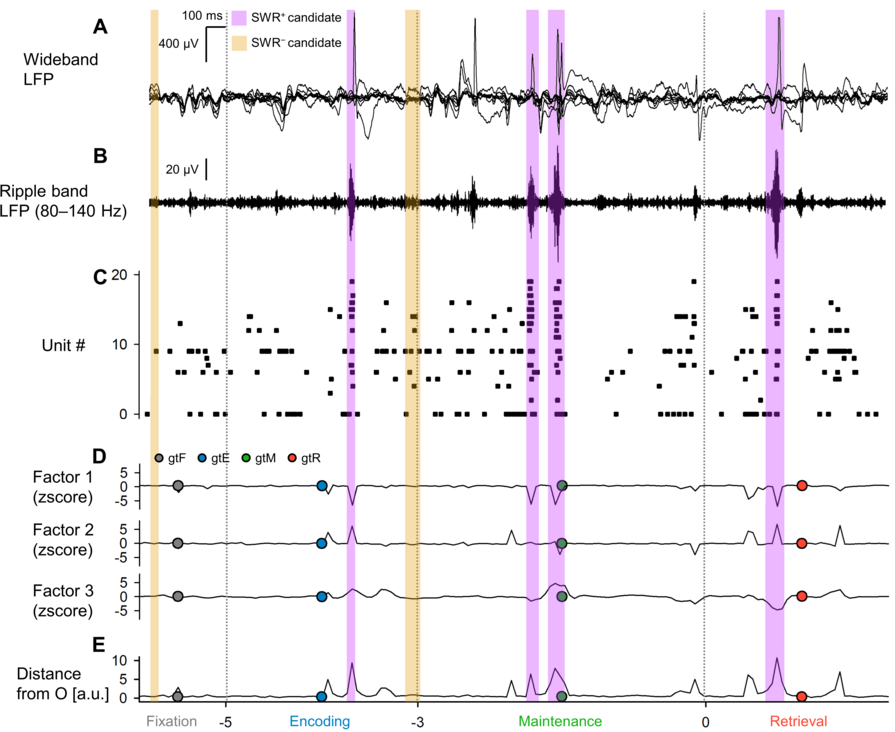
\includegraphics[width=1\textwidth]{./src/figures/.png/Figure_ID_01.png}
        	\caption{\DIFdelbeginFL \textbf{\DIFdelFL{Local Field Potentials, Multiunit Activity, and Neural Trajectories in the Hippocampus During a Modified Sternberg Task
}}
%DIFAUXCMD
\DIFdelendFL \DIFaddbeginFL \textbf{
\DIFaddFL{Local Field Potentials, Multiunit Activity, and Neural Trajectories in the Hippocampus during a Modified Sternberg Task
}}
\DIFaddendFL \smallskip
\\
\textbf{\textit{A.}} \DIFdelbeginFL \DIFdelFL{Representative }\DIFdelendFL \DIFaddbeginFL \DIFaddFL{Presented are representative }\DIFaddendFL wideband LFP signals for \DIFaddbeginFL \DIFaddFL{an }\DIFaddendFL intracranial EEG recording from the left hippocampal head\DIFdelbeginFL \DIFdelFL{are presented. This recording took place }\DIFdelendFL \DIFaddbeginFL \DIFaddFL{, obtained }\DIFaddendFL while the subject performed a modified Sternberg working memory task. \DIFdelbeginFL \DIFdelFL{Task }\DIFdelendFL \DIFaddbeginFL \DIFaddFL{The task comprises }\DIFaddendFL stages \DIFdelbeginFL \DIFdelFL{included }\DIFdelendFL \DIFaddbeginFL \DIFaddFL{of }\DIFaddendFL fixation (\DIFdelbeginFL \DIFdelFL{1 s}\DIFdelendFL \DIFaddbeginFL \DIFaddFL{1s}\DIFaddendFL , \textit{gray}), encoding (\DIFdelbeginFL \DIFdelFL{2 s}\DIFdelendFL \DIFaddbeginFL \DIFaddFL{2s}\DIFaddendFL , \textit{blue}), maintenance (\DIFdelbeginFL \DIFdelFL{3 s}\DIFdelendFL \DIFaddbeginFL \DIFaddFL{3s}\DIFaddendFL , \textit{green}), and retrieval (\DIFdelbeginFL \DIFdelFL{2 s}\DIFdelendFL \DIFaddbeginFL \DIFaddFL{2s}\DIFaddendFL , \textit{red}). \textbf{\textit{B.}} \DIFdelbeginFL \DIFdelFL{Displays }\DIFdelendFL \DIFaddbeginFL \DIFaddFL{Depicted are }\DIFaddendFL the associated ripple band LFP traces. \DIFdelbeginFL \DIFdelFL{Note }\DIFdelendFL \DIFaddbeginFL \DIFaddFL{Pay attention to the }\DIFaddendFL \textit{purple} and \textit{yellow} rectangles, which \DIFdelbeginFL \DIFdelFL{denote }\DIFdelendFL \DIFaddbeginFL \DIFaddFL{represent }\DIFaddendFL the timings for SWR$^+$ candidates and SWR$^-$ candidates, respectively (the latter \DIFdelbeginFL \DIFdelFL{serving }\DIFdelendFL \DIFaddbeginFL \DIFaddFL{serve }\DIFaddendFL as control events for SWR$^+$). \textbf{\textit{C.}} A raster plot \DIFdelbeginFL \DIFdelFL{illustrates }\DIFdelendFL \DIFaddbeginFL \DIFaddFL{demonstrates }\DIFaddendFL multi-unit spikes \DIFaddbeginFL \DIFaddFL{obtained }\DIFaddendFL from the LFP traces\DIFdelbeginFL \DIFdelFL{. These spikes have been }\DIFdelendFL \DIFaddbeginFL \DIFaddFL{, }\DIFaddendFL sorted using a spike algorithm \cite{niediek_reliable_2016}. \textbf{\textit{D.}} \DIFdelbeginFL \DIFdelFL{Shows }\DIFdelendFL \DIFaddbeginFL \DIFaddFL{The }\DIFaddendFL neural trajectories (NTs) \DIFdelbeginFL \DIFdelFL{computed }\DIFdelendFL \DIFaddbeginFL \DIFaddFL{calculated }\DIFaddendFL by GPFA\cite{yu_gaussian-process_2009} based on spike counts per unit with 50-ms bins \DIFdelbeginFL \DIFdelFL{. The }\DIFdelendFL \DIFaddbeginFL \DIFaddFL{are displayed; the }\DIFaddendFL geometric median of each phase is marked by dot circles. \textbf{\textit{E.}} \DIFdelbeginFL \DIFdelFL{Indicates the }\DIFdelendFL \DIFaddbeginFL \DIFaddFL{The }\DIFaddendFL distance of the NT from the origin point $O$ \DIFaddbeginFL \DIFaddFL{is shown}\DIFaddendFL .
}
% width=1\textwidth
        	\label{fig:01}
        \end{figure*}
        \clearpage
        \begin{figure*}[ht]
            \pdfbookmark[2]{ID 02}{figure_id_02}
        	\centering
            \DIFdelbeginFL %DIFDELCMD < \includegraphics[width=0.5\textwidth]{./src/figures/.png/Figure_ID_02.png}
%DIFDELCMD <         	%%%
\DIFdelendFL \DIFaddbeginFL \includegraphics[width=]{./src/figures/.png/Figure_ID_02.png}
        	\DIFaddendFL \caption{\DIFdelbeginFL \textbf{\DIFdelFL{State-Dependent Neural Trajectory of Hippocampal Neurons
}}
%DIFAUXCMD
\DIFdelendFL \DIFaddbeginFL \textbf{
\DIFaddFL{State-Dependent Neural Trajectories of Hippocampal Neurons
}}
\DIFaddendFL \smallskip
\\
\textbf{\textit{A.}} Neural trajectories (NTs) \DIFdelbeginFL \DIFdelFL{depicted }\DIFdelendFL \DIFaddbeginFL \DIFaddFL{are represented }\DIFaddendFL as a point cloud within the first three-dimensional factors derived from \DIFaddbeginFL \DIFaddFL{Gaussian Process Factor Analysis (}\DIFaddendFL GPFA\DIFaddbeginFL \DIFaddFL{) }\DIFaddendFL \cite{yu_gaussian-process_2009}. The smaller dots represent 50-ms NT bins, \DIFdelbeginFL \DIFdelFL{and }\DIFdelendFL \DIFaddbeginFL \DIFaddFL{while }\DIFaddendFL the larger dots with \DIFdelbeginFL \textit{\DIFdelFL{black}} %DIFAUXCMD
\DIFdelendFL \DIFaddbeginFL \DIFaddFL{black }\DIFaddendFL edges denote the geometric medians for each phase \DIFdelbeginFL \DIFdelFL{in }\DIFdelendFL \DIFaddbeginFL \DIFaddFL{of }\DIFaddendFL the Sternberg working memory task\DIFdelbeginFL \DIFdelFL{: }\DIFdelendFL \DIFaddbeginFL \DIFaddFL{. These phases include }\DIFaddendFL fixation ($\mathrm{\lVert g_{F} \rVert}$, \DIFdelbeginFL \textit{\DIFdelFL{gray}}%DIFAUXCMD
\DIFdelendFL \DIFaddbeginFL \DIFaddFL{gray}\DIFaddendFL ), encoding ($\mathrm{\lVert g_{E} \rVert}$, \DIFdelbeginFL \textit{\DIFdelFL{blue}}%DIFAUXCMD
\DIFdelendFL \DIFaddbeginFL \DIFaddFL{blue}\DIFaddendFL ), maintenance ($\mathrm{\lVert g_{M} \rVert}$, \DIFdelbeginFL \textit{\DIFdelFL{green}}%DIFAUXCMD
\DIFdelendFL \DIFaddbeginFL \DIFaddFL{green}\DIFaddendFL ), and retrieval ($\mathrm{\lVert g_{R} \rVert}$, \DIFdelbeginFL \textit{\DIFdelFL{red}}%DIFAUXCMD
\DIFdelendFL \DIFaddbeginFL \DIFaddFL{red}\DIFaddendFL ). \textbf{\textit{B.}} The figure \DIFdelbeginFL \DIFdelFL{presents }\DIFdelendFL \DIFaddbeginFL \DIFaddFL{shows }\DIFaddendFL the log-likelihood of \DIFdelbeginFL \DIFdelFL{the }\DIFdelendFL GPFA models \DIFdelbeginFL \DIFdelFL{versus }\DIFdelendFL \DIFaddbeginFL \DIFaddFL{against }\DIFaddendFL the number of dimensions used to embed multi-unit spikes found in the medial temporal lobe (MTL) regions. Specifically, the elbow method identified three as the optimal dimension. \textbf{\textit{C.}} This panel \DIFdelbeginFL \DIFdelFL{displays }\DIFdelendFL \DIFaddbeginFL \DIFaddFL{depicts }\DIFaddendFL the distance of the NTs from the origin ($O$) for the hippocampus (Hipp.), entorhinal cortex (EC), and amygdala (Amy.), plotted against the \DIFdelbeginFL \DIFdelFL{time }\DIFdelendFL elapsed \DIFdelbeginFL \DIFdelFL{from the }\DIFdelendFL \DIFaddbeginFL \DIFaddFL{time since }\DIFaddendFL probe onset. \textbf{\textit{D.}} \DIFdelbeginFL \DIFdelFL{The }\DIFdelendFL \DIFaddbeginFL \DIFaddFL{Here, the }\DIFaddendFL NT distance from $O$ within the MTL regions is \DIFdelbeginFL \DIFdelFL{shown}\DIFdelendFL \DIFaddbeginFL \DIFaddFL{displayed}\DIFaddendFL . The \DIFdelbeginFL \DIFdelFL{hippocampus has the }\DIFdelendFL greatest distance \DIFaddbeginFL \DIFaddFL{is in the hippocampus}\DIFaddendFL , followed by the EC and the Amygdala. \textbf{\textit{E.}} The box plot \DIFdelbeginFL \DIFdelFL{illustrates }\DIFdelendFL \DIFaddbeginFL \DIFaddFL{shows the }\DIFaddendFL inter-phase NT distances within the MTL regions.
}
        	%DIF <  width=0.5\textwidth
        	\label{fig:02}
        \end{figure*}
        \clearpage
        \begin{figure*}[ht]
            \pdfbookmark[2]{ID 03}{figure_id_03}
        	\centering
            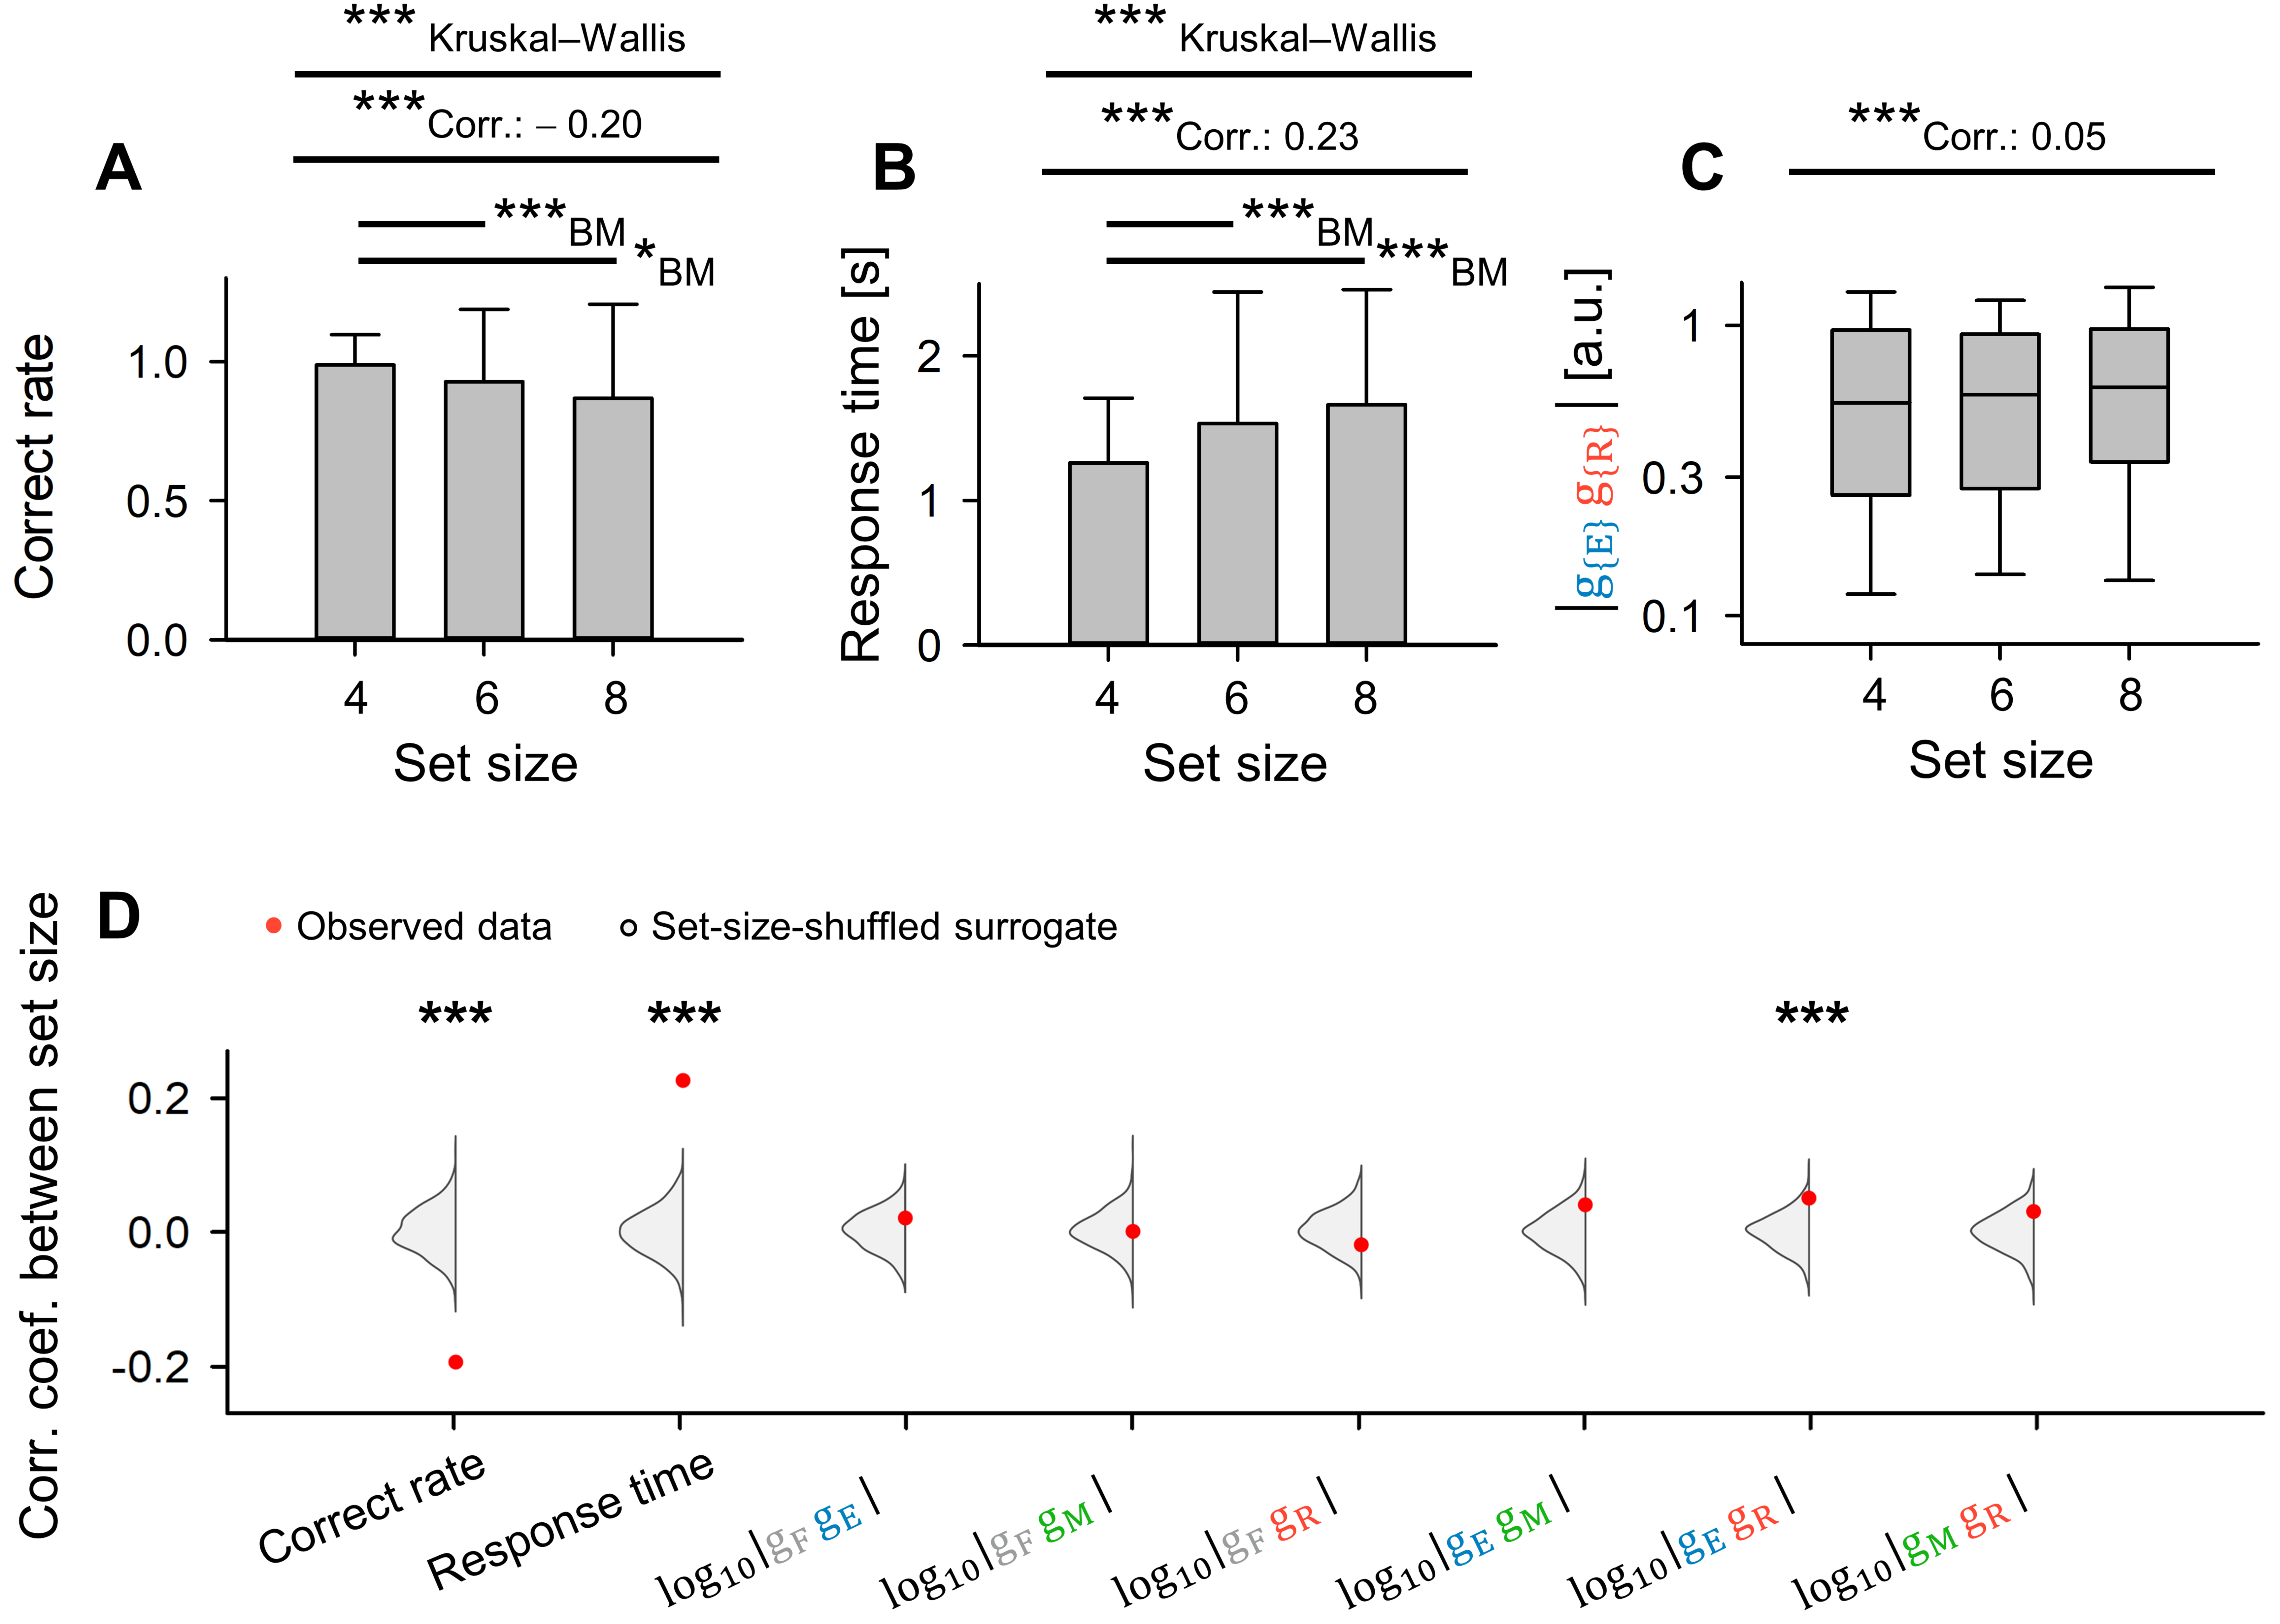
\includegraphics[width=1\textwidth]{./src/figures/.png/Figure_ID_03.png}
        	\caption{\DIFdelbeginFL \textbf{\DIFdelFL{Positive Correlation between Memory Load and Neural Trajectory Distance in the Hippocampus between Encoding and Retrieval Phases
}}
%DIFAUXCMD
\DIFdelendFL \DIFaddbeginFL \textbf{
\DIFaddFL{Positive Correlation Between Memory Load and Neural Trajectory Distance in the Hippocampus during Encoding and Retrieval Phases
}}
\DIFaddendFL \smallskip
\\
\textbf{\textit{A.}} \DIFdelbeginFL \DIFdelFL{The relationship }\DIFdelendFL \DIFaddbeginFL \DIFaddFL{Relationship }\DIFaddendFL between set size (number of \DIFdelbeginFL \DIFdelFL{letters to be }\DIFdelendFL encoded \DIFaddbeginFL \DIFaddFL{letters}\DIFaddendFL ) and accuracy in the working memory task (coefficient = $-0.20$, ***\textit{p} $<$ 0.001). \textbf{\textit{B.}} \DIFdelbeginFL \DIFdelFL{The correlation }\DIFdelendFL \DIFaddbeginFL \DIFaddFL{Correlation }\DIFaddendFL between set size and response time (coefficient = 0.23, ***\textit{p} $<$ 0.001). \textbf{\textit{C.}} \DIFdelbeginFL \DIFdelFL{The correlation between }\DIFdelendFL \DIFaddbeginFL \DIFaddFL{Correlation of }\DIFaddendFL set size \DIFdelbeginFL \DIFdelFL{on }\DIFdelendFL \DIFaddbeginFL \DIFaddFL{with }\DIFaddendFL the inter-phase distances between \DIFdelbeginFL \DIFdelFL{the }\DIFdelendFL encoding and retrieval phases ($\lVert \mathrm{g_{E}g_{R}} \rVert$) (correlation coefficient = 0.05, ***\textit{p} $<$ 0.001). \textbf{\textit{D.}} Experimental \DIFdelbeginFL \DIFdelFL{observations of }\DIFdelendFL correlations between set size and the following parameters: accuracy, response time, $\log_{10}{\lVert \mathrm{g_{F}g_{E}} \rVert}$, $\log_{10}{\lVert \mathrm{g_{F}g_{M}} \rVert}$, $\log_{10}{\lVert \mathrm{g_{F}g_{R}} \rVert}$, $\log_{10}{\lVert \mathrm{g_{E}g_{M}} \rVert}$, $\log_{10}{\lVert \mathrm{g_{E}g_{R}} \rVert}$, and $\log_{10}{\lVert \mathrm{g_{M}g_{R}} \rVert}$ represented by \textit{red} dots. The kernel density plots (\textit{gray}) illustrate the corresponding shuffled surrogate with set size (\textit{n} = 1,000) (***\textit{p}s $<$ 0.001).
}
% width=1\textwidth
        	\label{fig:03}
        \end{figure*}
        \clearpage
        \begin{figure*}[ht]
            \pdfbookmark[2]{ID 04}{figure_id_04}
        	\centering
            \includegraphics[width=1\textwidth]{./src/figures/.png/Figure_ID_04.png}
        	\caption{\DIFdelbeginFL \textbf{\DIFdelFL{Detection of SWRs in Putative CA1 Regions}}%DIFAUXCMD
\DIFdelendFL \DIFaddbeginFL \textbf{\DIFaddFL{Detection of Sharp Wave Ripples in Presumed CA1 Regions}}\DIFaddendFL \\
\textbf{\textit{A.}} \DIFdelbeginFL \DIFdelFL{Two-dimensional }\DIFdelendFL \DIFaddbeginFL \DIFaddFL{A two-dimensional }\DIFaddendFL UMAP \cite{mcinnes_umap_2018} projection \DIFdelbeginFL \DIFdelFL{displays }\DIFdelendFL \DIFaddbeginFL \DIFaddFL{illustrates }\DIFaddendFL multi-unit spikes during \DIFaddbeginFL \DIFaddFL{positive sharp wave ripples (}\DIFaddendFL SWR$^+$\DIFaddbeginFL \DIFaddFL{) }\DIFaddendFL candidates (\textit{purple}) and \DIFaddbeginFL \DIFaddFL{negative sharp wave ripples (}\DIFaddendFL SWR$^-$\DIFaddbeginFL \DIFaddFL{) }\DIFaddendFL candidates (\textit{yellow}). \textbf{\textit{B.}} A cumulative density plot \DIFdelbeginFL \DIFdelFL{indicates }\DIFdelendFL \DIFaddbeginFL \DIFaddFL{shows }\DIFaddendFL silhouette scores, \DIFdelbeginFL \DIFdelFL{reflecting }\DIFdelendFL \DIFaddbeginFL \DIFaddFL{which reflect the quality of }\DIFaddendFL UMAP clustering \DIFdelbeginFL \DIFdelFL{quality }\DIFdelendFL (\DIFdelbeginFL \DIFdelFL{see }\DIFdelendFL \DIFaddbeginFL \DIFaddFL{refer to }\DIFaddendFL Table~\ref{tab:02}). \DIFdelbeginFL \DIFdelFL{Hippocampal }\DIFdelendFL \DIFaddbeginFL \DIFaddFL{Presumed CA1 }\DIFaddendFL regions \DIFdelbeginFL \DIFdelFL{with }\DIFdelendFL \DIFaddbeginFL \DIFaddFL{are identified by }\DIFaddendFL silhouette scores \DIFdelbeginFL \DIFdelFL{exceeding }\DIFdelendFL \DIFaddbeginFL \DIFaddFL{greater than }\DIFaddendFL 0.60 (equivalent to the \DIFdelbeginFL \DIFdelFL{$75^{th}$ }\DIFdelendFL \DIFaddbeginFL \DIFaddFL{75th }\DIFaddendFL percentile)\DIFdelbeginFL \DIFdelFL{are identified as putative CA1 regions}\DIFdelendFL . \DIFdelbeginFL \DIFdelFL{SWR$^+$ }\DIFdelendFL \DIFaddbeginFL \DIFaddFL{Hits }\DIFaddendFL and \DIFdelbeginFL \DIFdelFL{SWR$^-$ candidates, which were }\DIFdelendFL \DIFaddbeginFL \DIFaddFL{misses }\DIFaddendFL recorded from these regions \DIFdelbeginFL \DIFdelFL{, }\DIFdelendFL are classified as SWR$^+$ and SWR$^-$ \DIFdelbeginFL \DIFdelFL{respectively }\DIFdelendFL \DIFaddbeginFL \DIFaddFL{accordingly }\DIFaddendFL (\textit{n}s = 1,170). \textbf{\textit{C.}} \DIFdelbeginFL \DIFdelFL{Identical }\DIFdelendFL \DIFaddbeginFL \DIFaddFL{Consistent }\DIFaddendFL distributions of durations \DIFdelbeginFL \DIFdelFL{are presented }\DIFdelendFL for SWR$^+$ (\textit{purple}) and SWR$^-$ (\textit{yellow}) \DIFaddbeginFL \DIFaddFL{are demonstrated}\DIFaddendFL , \DIFdelbeginFL \DIFdelFL{based on their definitions }\DIFdelendFL \DIFaddbeginFL \DIFaddFL{as defined by the median interquartile range }\DIFaddendFL (\DIFaddbeginFL \DIFaddFL{IQR) of }\DIFaddendFL 93.0 [65.4] ms\DIFdelbeginFL \DIFdelFL{, median }%DIFDELCMD < [%%%
\DIFdelFL{IQR}%DIFDELCMD < ]%%%
\DIFdelFL{)}\DIFdelendFL . \textbf{\textit{D.}} \DIFdelbeginFL \DIFdelFL{SWR incidence for both }\DIFdelendFL \DIFaddbeginFL \DIFaddFL{The occurrence of }\DIFaddendFL SWR$^+$ (\textit{purple}) and SWR$^-$ (\textit{yellow}), \DIFdelbeginFL \DIFdelFL{relative }\DIFdelendFL \DIFaddbeginFL \DIFaddFL{in relation }\DIFaddendFL to the probe's timing, is \DIFdelbeginFL \DIFdelFL{illustrated }\DIFdelendFL \DIFaddbeginFL \DIFaddFL{depicted }\DIFaddendFL as a mean \textpm 95\% confidence interval. \DIFdelbeginFL \DIFdelFL{However, }\DIFdelendFL \DIFaddbeginFL \DIFaddFL{Please note that the }\DIFaddendFL intervals may not be visibly \DIFdelbeginFL \DIFdelFL{apparent }\DIFdelendFL \DIFaddbeginFL \DIFaddFL{discernible }\DIFaddendFL due to their confined ranges, \DIFdelbeginFL \DIFdelFL{be aware that }\DIFdelendFL \DIFaddbeginFL \DIFaddFL{despite }\DIFaddendFL a significant \DIFaddbeginFL \DIFaddFL{surge in }\DIFaddendFL SWR incidence \DIFdelbeginFL \DIFdelFL{increase was detected }\DIFdelendFL during the initial 400 ms of the retrieval phase (0.421 [Hz], *\textit{p} $<$ 0.05, bootstrap test). \textbf{\textit{E.}} \DIFdelbeginFL \DIFdelFL{Distributions }\DIFdelendFL \DIFaddbeginFL \DIFaddFL{The distributions }\DIFaddendFL of ripple band peak amplitudes for SWR$^-$ (\textit{yellow}; 2.37 [0.33] SD of baseline, median [IQR]) and SWR$^+$ (\textit{purple}; 3.05 [0.85] SD of baseline, median [IQR]) are \DIFdelbeginFL \DIFdelFL{manifested }\DIFdelendFL \DIFaddbeginFL \DIFaddFL{depicted }\DIFaddendFL (***\textit{p} $<$ 0.001, the Brunner--Munzel test).} % width=1\textwidth
        	\label{fig:04}
        \end{figure*}
        \clearpage
        \begin{figure*}[ht]
            \pdfbookmark[2]{ID 05}{figure_id_05}
        	\centering
            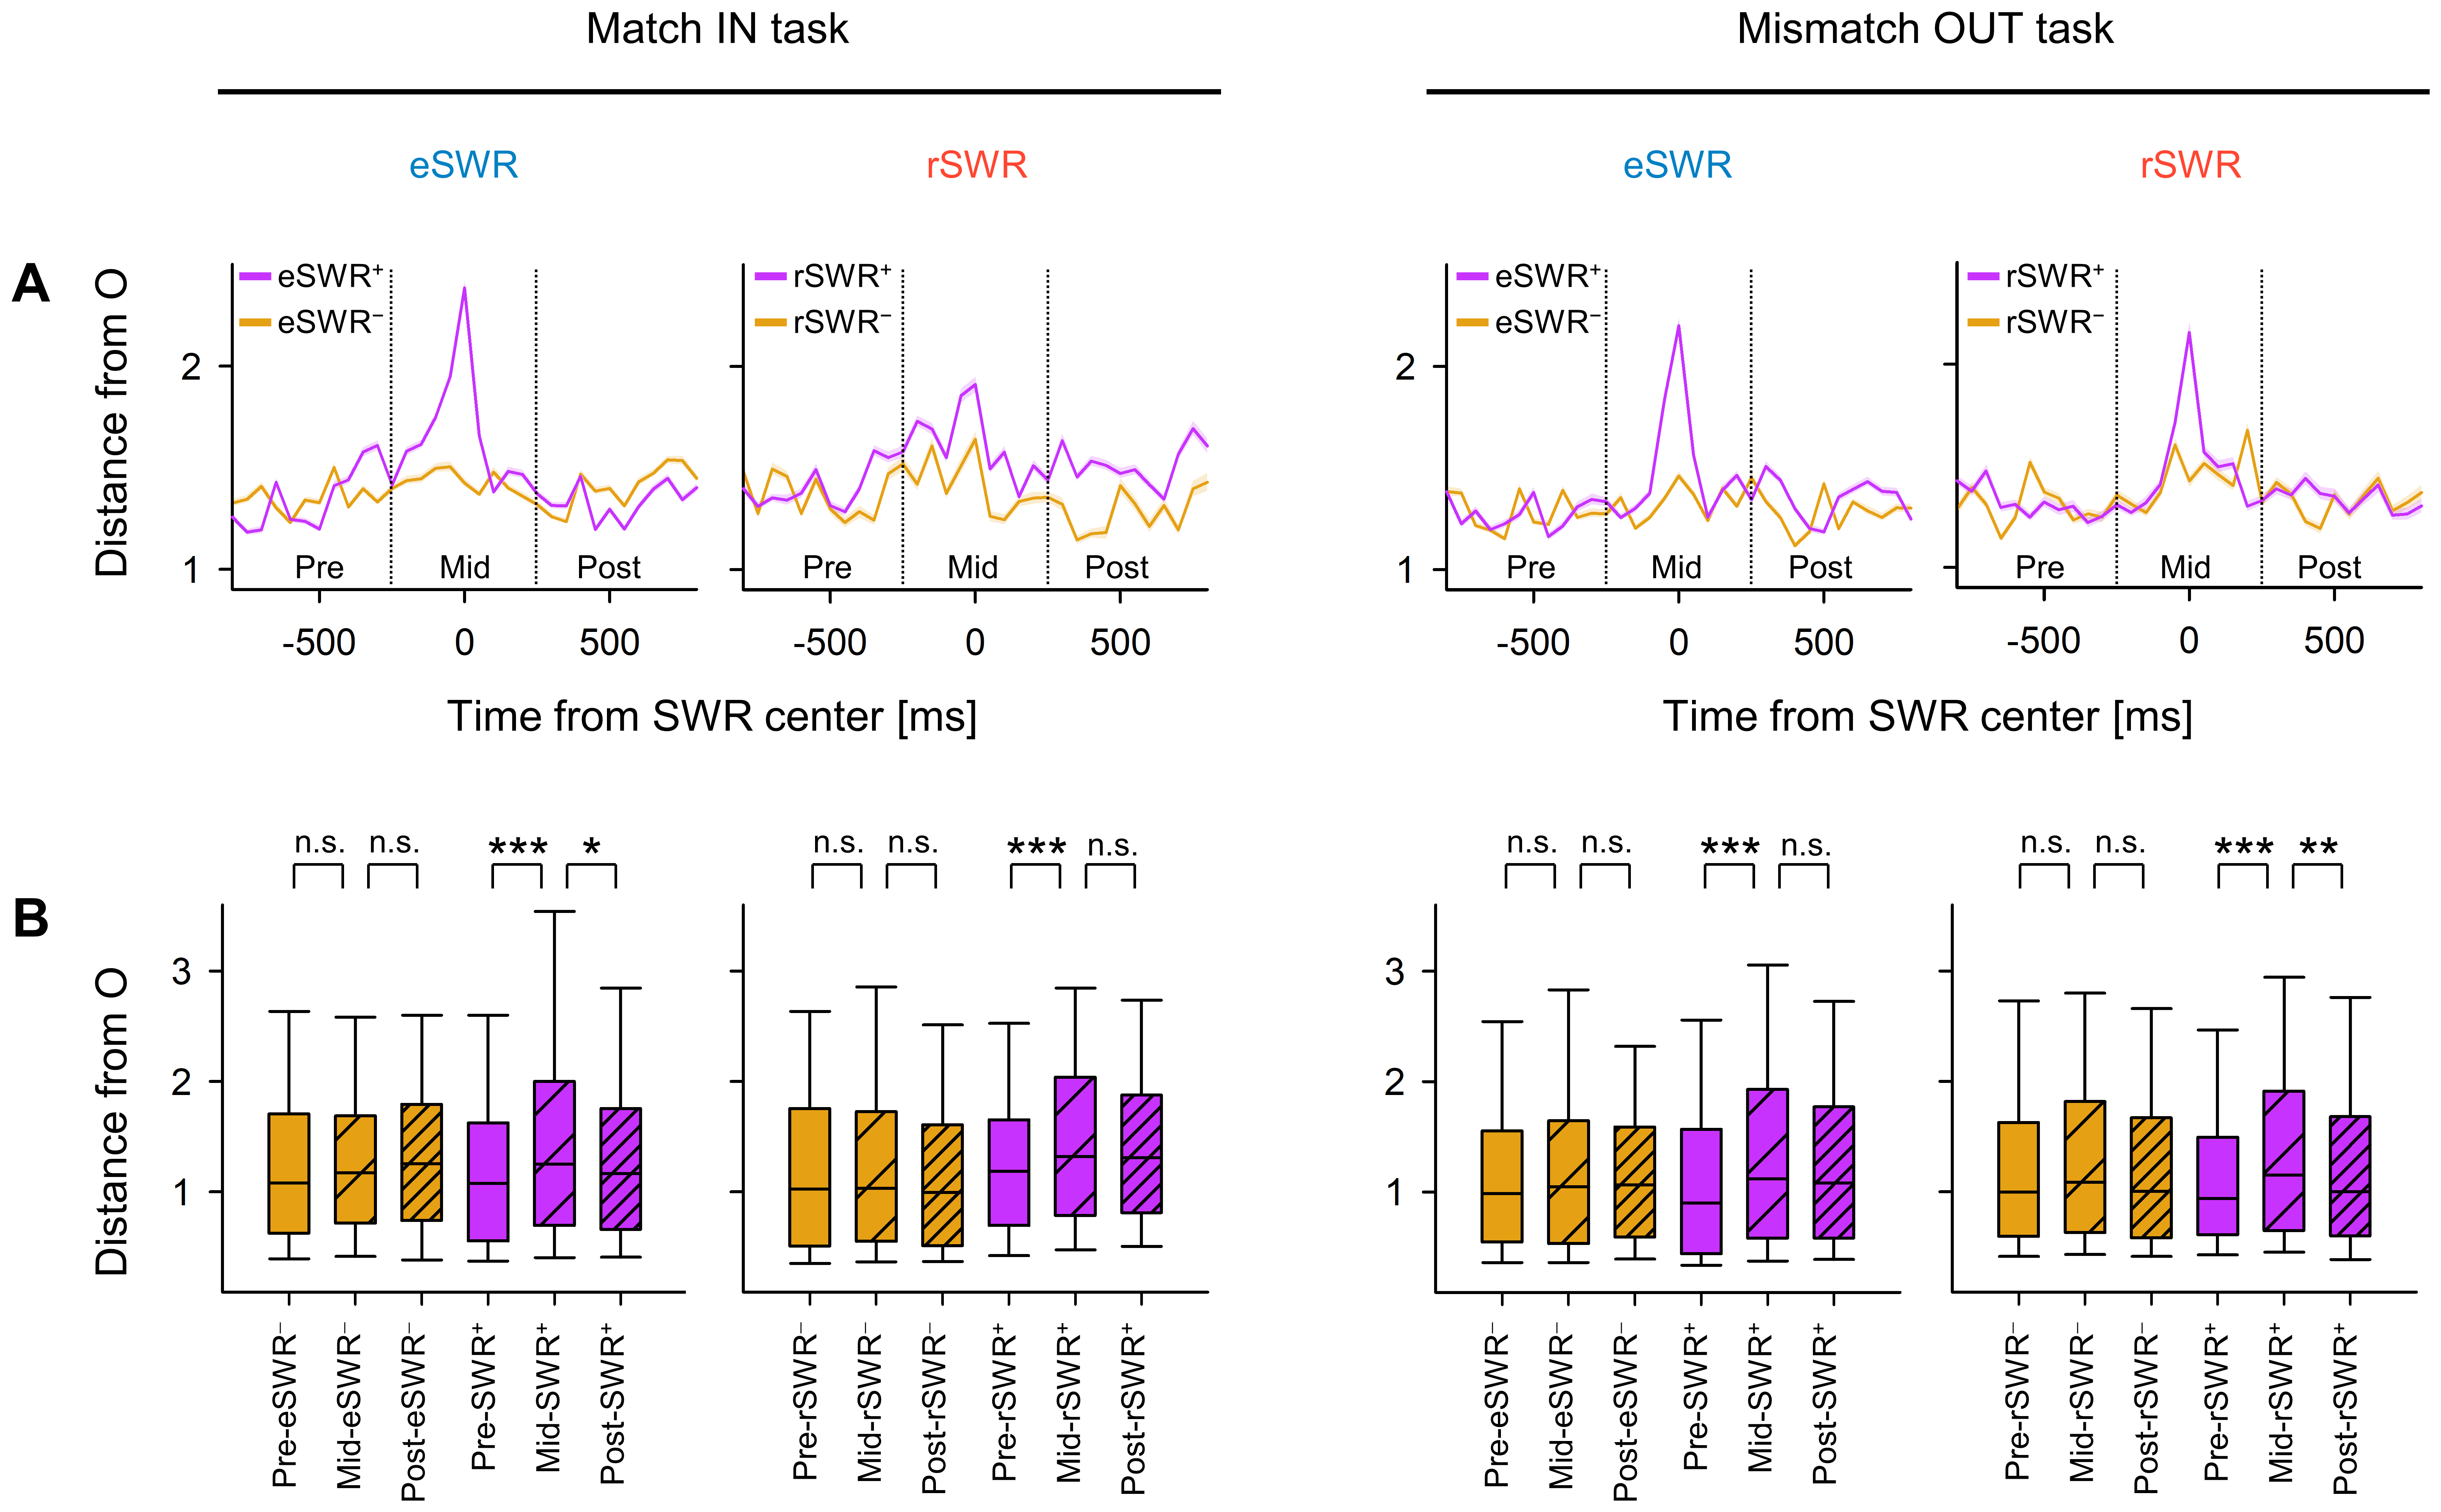
\includegraphics[width=1\textwidth]{./src/figures/.png/Figure_ID_05.png}
        	\caption{\DIFdelbeginFL \textbf{\DIFdelFL{Transient Change in Neural Trajectory during SWR}}
%DIFAUXCMD
\DIFdelendFL \DIFaddbeginFL \textbf{\DIFaddFL{Transient Change in Neural Trajectory during Sharp-Wave Ripple Events}}
\DIFaddendFL \smallskip
\\
\textbf{\textit{A.}} \DIFdelbeginFL \DIFdelFL{The distance }\DIFdelendFL \DIFaddbeginFL \DIFaddFL{Distance }\DIFaddendFL from origin ($O$) of the peri-sharp-wave-ripple neural trajectory (mean \textpm 95\% confidence interval). \DIFdelbeginFL \DIFdelFL{The intervals }\DIFdelendFL \DIFaddbeginFL \DIFaddFL{Intervals }\DIFaddendFL may be \DIFdelbeginFL \DIFdelFL{obscured }\DIFdelendFL \DIFaddbeginFL \DIFaddFL{inconspicuous }\DIFaddendFL due to their minimal ranges. \textbf{\textit{B.}} \DIFdelbeginFL \DIFdelFL{The distance }\DIFdelendFL \DIFaddbeginFL \DIFaddFL{Distance }\DIFaddendFL from the origin ($O$) during the pre-, mid-, and \DIFdelbeginFL \DIFdelFL{post-SWR }\DIFdelendFL \DIFaddbeginFL \DIFaddFL{post-sharp-wave ripple }\DIFaddendFL periods is demonstrated (*\textit{p} $<$ 0.05, **\textit{p} $<$ 0.01, ***\textit{p} $<$ 0.001; Brunner--Munzel test applied). Abbreviations: SWR, sharp-wave ripple \DIFdelbeginFL \DIFdelFL{events}\DIFdelendFL \DIFaddbeginFL \DIFaddFL{event}\DIFaddendFL ; eSWR, \DIFdelbeginFL \DIFdelFL{SWR }\DIFdelendFL \DIFaddbeginFL \DIFaddFL{sharp-wave ripple }\DIFaddendFL during the encoding phase; rSWR, \DIFdelbeginFL \DIFdelFL{SWR }\DIFdelendFL \DIFaddbeginFL \DIFaddFL{sharp-wave ripple }\DIFaddendFL within the retrieval phase; SWR$^+$, positive \DIFdelbeginFL \DIFdelFL{SWR }\DIFdelendFL \DIFaddbeginFL \DIFaddFL{sharp-wave ripple }\DIFaddendFL event; SWR$^-$, control events for SWR$^+$; pre-, mid-, or post-SWR refer to the time intervals from $-800$ to $-250$ ms, from $-250$ to $+250$ ms, or from $+250$ to $+800$ ms, respectively, all relative to the \DIFdelbeginFL \DIFdelFL{SWR }\DIFdelendFL center \DIFaddbeginFL \DIFaddFL{of the sharp-wave ripple event}\DIFaddendFL .}
% width=1\textwidth
        	\label{fig:05}
        \end{figure*}
        \clearpage
        \begin{figure*}[ht]
            \pdfbookmark[2]{ID 06}{figure_id_06}
        	\centering
            \DIFdelbeginFL %DIFDELCMD < 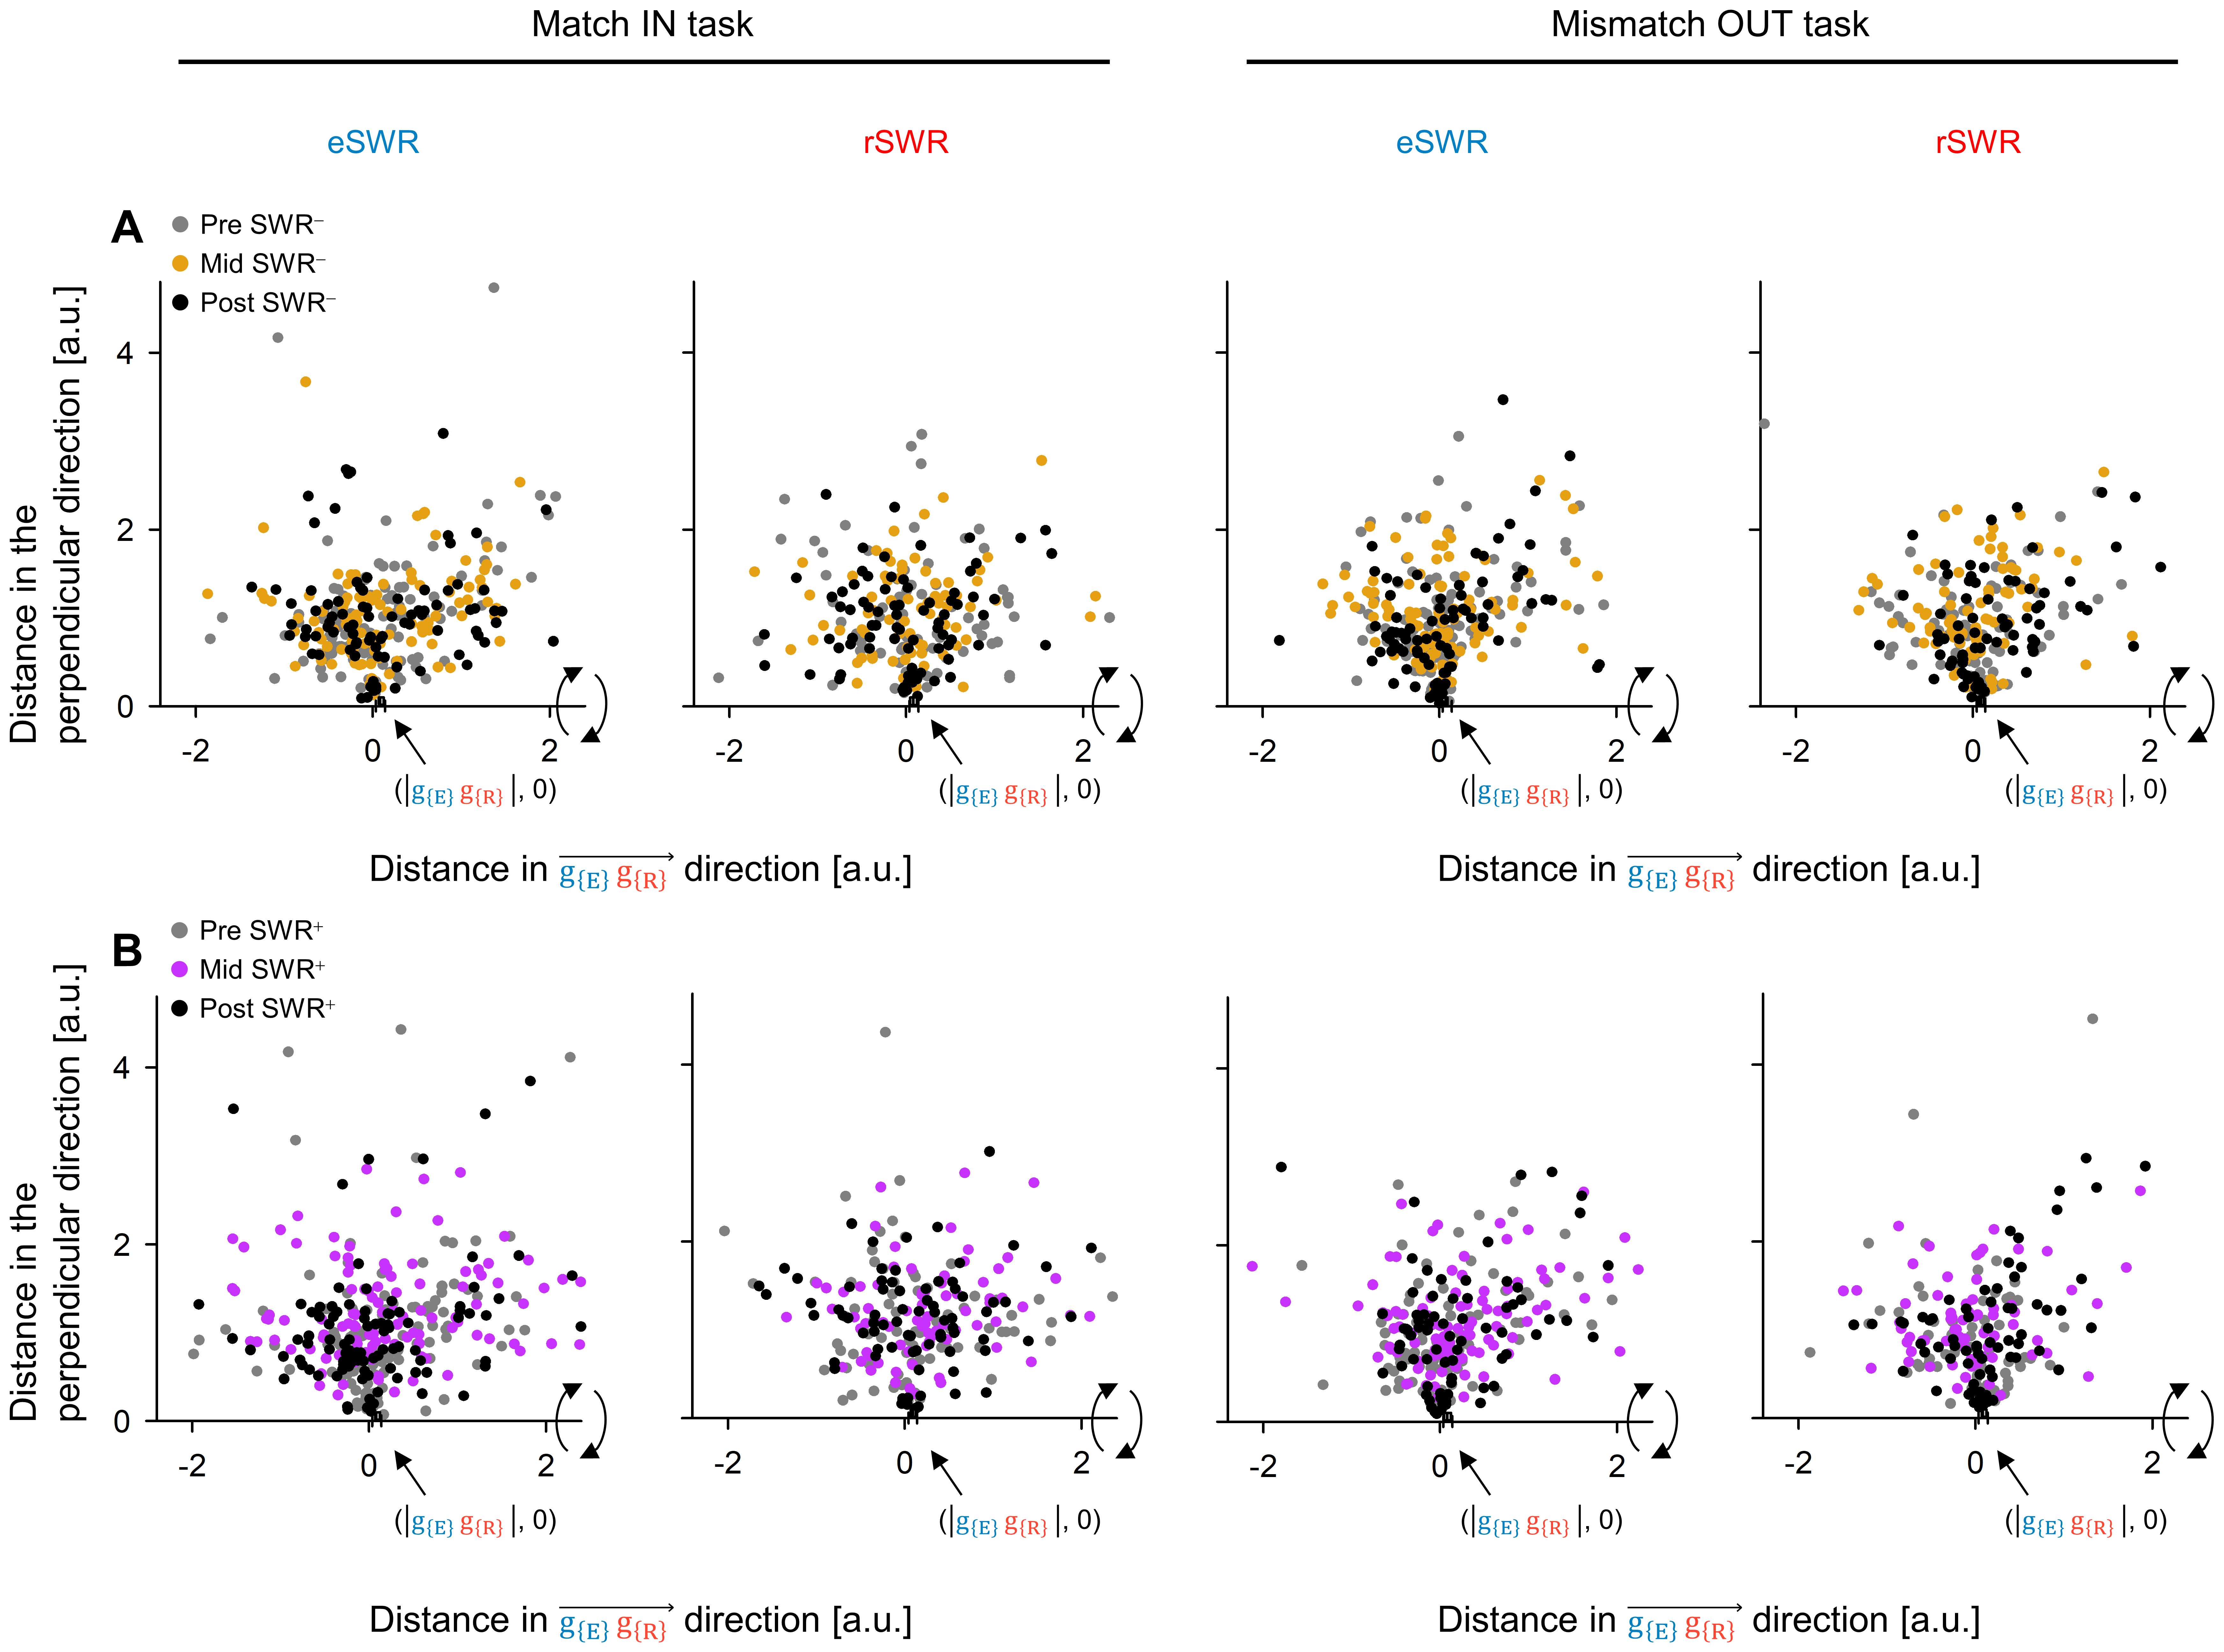
\includegraphics[width=1\textwidth]{./src/figures/.png/Figure_ID_06.png}
%DIFDELCMD <         	%%%
\DIFdelendFL \DIFaddbeginFL 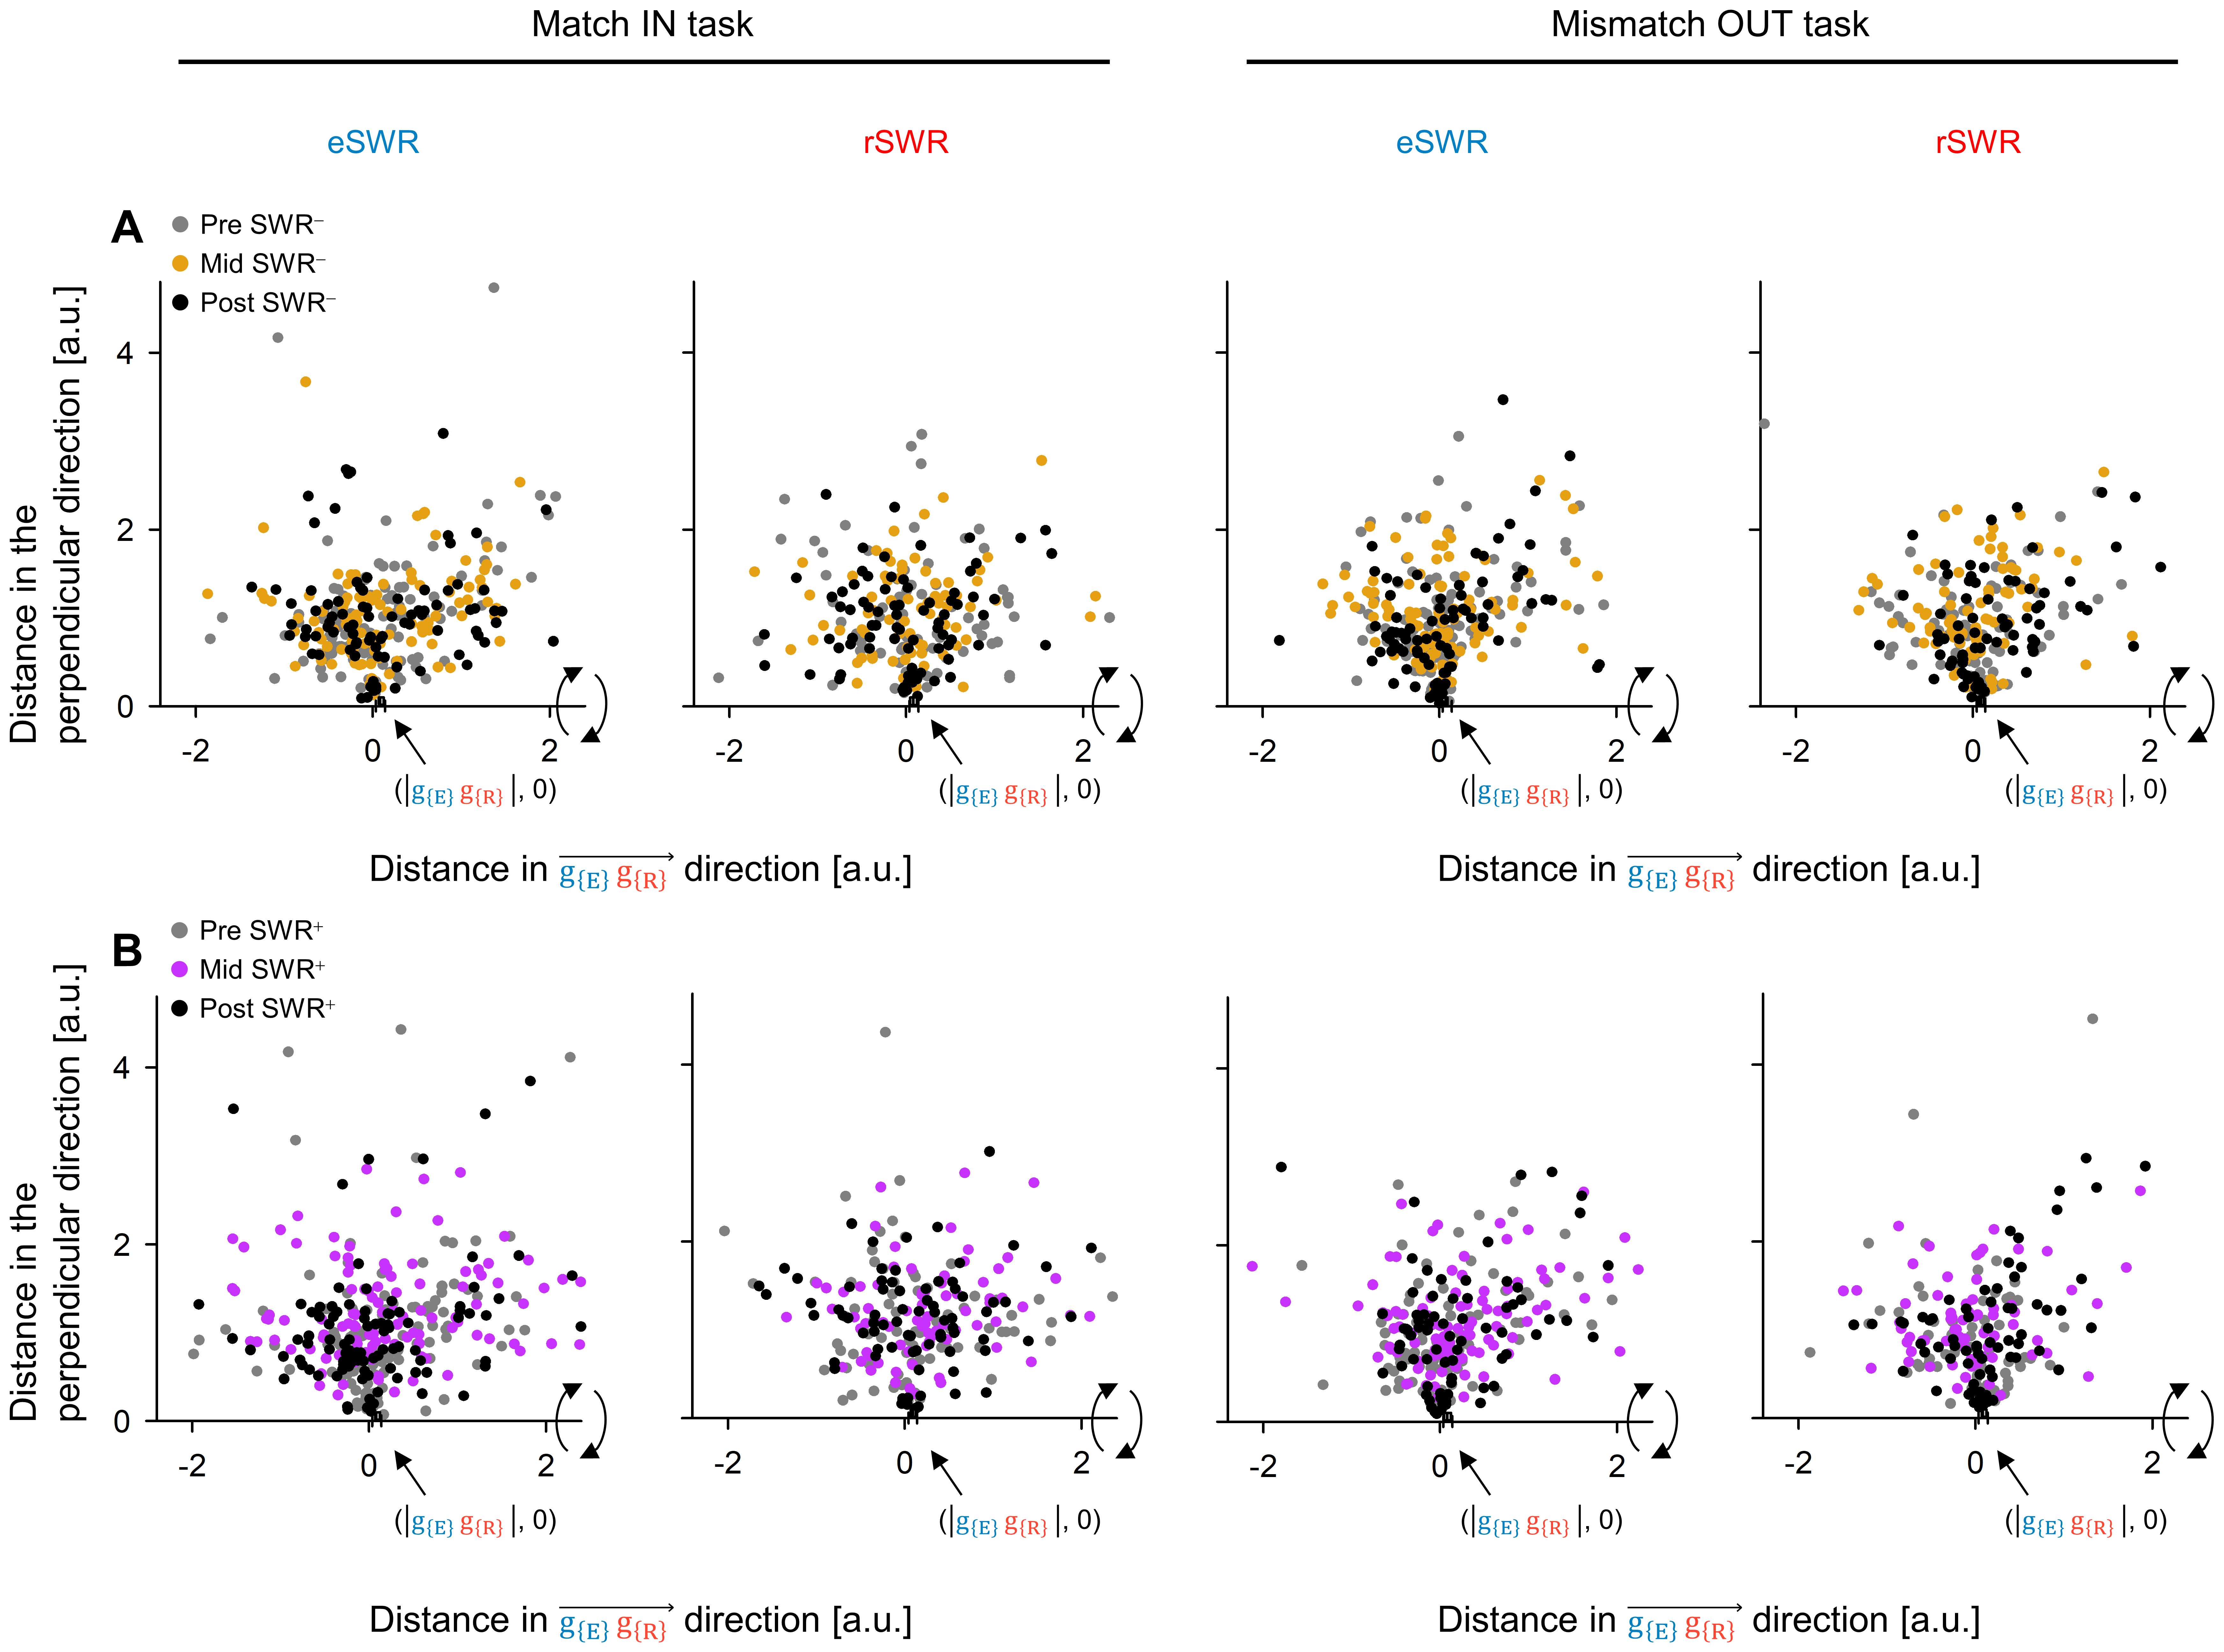
\includegraphics[width=]{./src/figures/.png/Figure_ID_06.png}
        	\DIFaddendFL \caption{\DIFdelbeginFL \textbf{\DIFdelFL{Visualization of Neural Trajectory During SWR in Two-Dimensional Space
}}
%DIFAUXCMD
\DIFdelendFL \DIFaddbeginFL \textbf{\DIFaddFL{Visualization of Neural Trajectories during Sharp-Wave Ripple Events in Two-Dimensional Space}}
\DIFaddendFL \smallskip
\\
The panels \DIFdelbeginFL \DIFdelFL{depict }\DIFdelendFL \DIFaddbeginFL \DIFaddFL{portray }\DIFaddendFL hippocampal neural trajectories (NTs) during \DIFaddbeginFL \DIFaddFL{sharp-wave ripple (}\DIFaddendFL SWR\DIFaddbeginFL \DIFaddFL{) events, }\DIFaddendFL projected onto two-dimensional spaces. \textbf{\textit{A.}} \DIFdelbeginFL \DIFdelFL{Shows }\DIFdelendFL \DIFaddbeginFL \DIFaddFL{Displays }\DIFaddendFL the hippocampal NTs as point clouds during pre-SWR$^-$ (\DIFdelbeginFL \textit{\DIFdelFL{gray}}%DIFAUXCMD
\DIFdelendFL \DIFaddbeginFL \DIFaddFL{in gray}\DIFaddendFL ), mid-SWR$^-$ (\DIFdelbeginFL \textit{\DIFdelFL{yellow}}%DIFAUXCMD
\DIFdelendFL \DIFaddbeginFL \DIFaddFL{in yellow}\DIFaddendFL ), and post-SWR$^-$ (\DIFdelbeginFL \textit{\DIFdelFL{black}}%DIFAUXCMD
\DIFdelendFL \DIFaddbeginFL \DIFaddFL{in black}\DIFaddendFL ). \textbf{\textit{B.}} \DIFdelbeginFL \DIFdelFL{Conveys }\DIFdelendFL \DIFaddbeginFL \DIFaddFL{Presents }\DIFaddendFL the \DIFdelbeginFL \DIFdelFL{equivalent }\DIFdelendFL \DIFaddbeginFL \DIFaddFL{comparable depiction }\DIFaddendFL for SWR$^+$ \DIFdelbeginFL \DIFdelFL{rather than }\DIFdelendFL \DIFaddbeginFL \DIFaddFL{instead of }\DIFaddendFL SWR$^-$. The projection was \DIFdelbeginFL \DIFdelFL{executed }\DIFdelendFL \DIFaddbeginFL \DIFaddFL{undertaken }\DIFaddendFL as follows: \DIFdelbeginFL \DIFdelFL{First}\DIFdelendFL \DIFaddbeginFL \DIFaddFL{Firstly}\DIFaddendFL , a linear transformation \DIFdelbeginFL \DIFdelFL{placed }\DIFdelendFL \DIFaddbeginFL \DIFaddFL{set }\DIFaddendFL $\mathrm{g_{E}}$ at the origin \DIFaddbeginFL \DIFaddFL{point }\DIFaddendFL $O$ (0,0), and $\mathrm{g_{R}}$ at ($\lVert \mathrm{g_{E}g_{R}} \rVert$, 0). \DIFdelbeginFL \DIFdelFL{The }\DIFdelendFL \DIFaddbeginFL \DIFaddFL{Subsequently, the }\DIFaddendFL point cloud was \DIFdelbeginFL \DIFdelFL{subsequently }\DIFdelendFL rotated around the $\mathrm{g_{E}g_{R}}$ axis (\DIFdelbeginFL \DIFdelFL{similar }\DIFdelendFL \DIFaddbeginFL \DIFaddFL{akin }\DIFaddendFL to the \DIFdelbeginFL \DIFdelFL{x axis}\DIFdelendFL \DIFaddbeginFL \DIFaddFL{x-axis}\DIFaddendFL )\DIFdelbeginFL \DIFdelFL{for adaptation }\DIFdelendFL \DIFaddbeginFL \DIFaddFL{, adjusting it }\DIFaddendFL to two-dimensional spaces. \DIFdelbeginFL \DIFdelFL{Thus}\DIFdelendFL \DIFaddbeginFL \DIFaddFL{As such}\DIFaddendFL , \DIFdelbeginFL \DIFdelFL{within }\DIFdelendFL \DIFaddbeginFL \DIFaddFL{in }\DIFaddendFL these two-dimensional spaces, the distances from point $O$ and the angles for the $\mathrm{g_{E}g_{R}}$ axis are \DIFdelbeginFL \DIFdelFL{retained }\DIFdelendFL \DIFaddbeginFL \DIFaddFL{preserved identically }\DIFaddendFL as in the original three-dimensional spaces \DIFdelbeginFL \DIFdelFL{created }\DIFdelendFL \DIFaddbeginFL \DIFaddFL{generated }\DIFaddendFL by \DIFaddbeginFL \DIFaddFL{Gaussian Process Factor Analysis (}\DIFaddendFL GPFA\DIFaddbeginFL \DIFaddFL{)}\DIFaddendFL . Abbreviations: SWR denotes sharp-wave ripple events; \DIFaddbeginFL \DIFaddFL{encoding sharp-wave ripple (}\DIFaddendFL eSWR\DIFaddbeginFL \DIFaddFL{) }\DIFaddendFL refers to SWR during the encoding phase; \DIFaddbeginFL \DIFaddFL{retrieval sharp-wave ripple (}\DIFaddendFL rSWR\DIFdelbeginFL \DIFdelFL{signals }\DIFdelendFL \DIFaddbeginFL \DIFaddFL{) indicates }\DIFaddendFL SWR during the retrieval phase; SWR$^+$ \DIFdelbeginFL \DIFdelFL{, }\DIFdelendFL characterizes \DIFdelbeginFL \DIFdelFL{an }\DIFdelendFL \DIFaddbeginFL \DIFaddFL{a }\DIFaddendFL SWR event; SWR$^-$ \DIFdelbeginFL \DIFdelFL{signifies }\DIFdelendFL \DIFaddbeginFL \DIFaddFL{designates }\DIFaddendFL control events for SWR$^+$; pre-SWR, mid-SWR, or post-SWR \DIFdelbeginFL \DIFdelFL{, represent }\DIFdelendFL \DIFaddbeginFL \DIFaddFL{define }\DIFaddendFL the time intervals from $-800$ to $-250$ ms, from $-250$ to $+250$ ms, or from $+250$ to $+800$ ms from the center of \DIFdelbeginFL \DIFdelFL{the }\DIFdelendFL SWR\DIFaddbeginFL \DIFaddFL{, respectively}\DIFaddendFL .
}
        	%DIF <  width=1\textwidth
        	\label{fig:06}
        \end{figure*}
        \clearpage
        \begin{figure*}[ht]
            \pdfbookmark[2]{ID 07}{figure_id_07}
        	\centering
            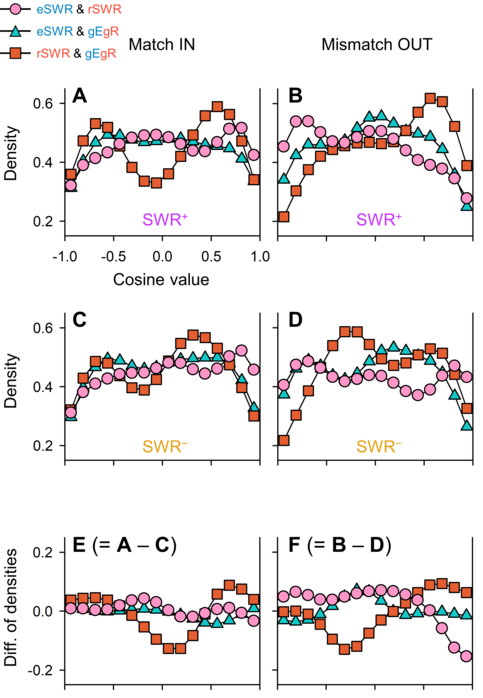
\includegraphics[width=0.5\textwidth]{./src/figures/.png/Figure_ID_07.png}
        	\caption{\DIFdelbeginFL \textbf{\DIFdelFL{Direction of Neural Trajectory During SWR Based on Encoding and Retrieval States
}}
%DIFAUXCMD
\DIFdelendFL \DIFaddbeginFL \textbf{
\DIFaddFL{Direction of Neural Trajectory during SWR Based on Encoding and Retrieval States
}}
\DIFaddendFL \smallskip
\\
\textbf{\textit{A--B}} The kernel density estimation distributions of $\protect\overrightarrow{{\mathrm{eSWR^+}}}$ $\cdot$ $\protect\overrightarrow{{\mathrm{rSWR^+}}}$ (\textit{pink circles}), $\protect\overrightarrow{{\mathrm{eSWR^+}}}$ $\cdot$ $\protect\overrightarrow{{\mathrm{g_{E}g_{R}}}}$ (\textit{blue triangles}), and $\protect\overrightarrow{{\mathrm{rSWR^+}}}$ $\cdot$ $\protect\overrightarrow{{\mathrm{g_{E}g_{R}}}}$ (\textit{red rectangles}) in Match In (\textit{A}) and Mismatch OUT tasks (\textit{B}). \textbf{\textit{C--D}} The corresponding distributions of $\mathrm{SWR^-}$ \DIFdelbeginFL \DIFdelFL{instead of }\DIFdelendFL \DIFaddbeginFL \DIFaddFL{to }\DIFaddendFL those of $\mathrm{SWR^+}$ in \textit{A} and \textit{B}. \textbf{\textit{E--F}} The \DIFdelbeginFL \DIFdelFL{differences in the }\DIFdelendFL \DIFaddbeginFL \DIFaddFL{differential }\DIFaddendFL distributions of $\mathrm{SWR^+}$ and \DIFdelbeginFL \DIFdelFL{those of }\DIFdelendFL $\mathrm{SWR^-}$, \DIFdelbeginFL \DIFdelFL{showing }\DIFdelendFL \DIFaddbeginFL \DIFaddFL{demonstrating }\DIFaddendFL SWR components (\textit{E} = \textit{C} - \textit{A}\DIFdelbeginFL \DIFdelFL{\& }\DIFdelendFL \DIFaddbeginFL \DIFaddFL{, }\DIFaddendFL \textit{F} = \textit{D} - \textit{B}). Biphasic distributions of $\protect\overrightarrow{{\mathrm{rSWR^-}}}$ $\cdot$ $\protect\overrightarrow{{\mathrm{g_{E}g_{R}}}}$ \DIFdelbeginFL \DIFdelFL{indicate }\DIFdelendFL \DIFaddbeginFL \DIFaddFL{signal }\DIFaddendFL fluctuations between the encoding and retrieval states during the Sternberg task. \DIFdelbeginFL \DIFdelFL{Also, contradicting }\DIFdelendFL \DIFaddbeginFL \DIFaddFL{A contrasting }\DIFaddendFL directionality between $\protect\overrightarrow{{\mathrm{eSWR^+}}}$ and $\protect\overrightarrow{{\mathrm{rSWR^+}}}$ \DIFdelbeginFL \DIFdelFL{was observed }\DIFdelendFL \DIFaddbeginFL \DIFaddFL{is noticeable }\DIFaddendFL (pink circles) not in \DIFaddbeginFL \DIFaddFL{the }\DIFaddendFL Match IN task (\textbf{\textit{E}}), but in \DIFaddbeginFL \DIFaddFL{the }\DIFaddendFL Mismatch OUT task (\textbf{\textit{F}}). Lastly, transitions from the retrieval to encoding states are \DIFdelbeginFL \DIFdelFL{evident }\DIFdelendFL \DIFaddbeginFL \DIFaddFL{apparent }\DIFaddendFL in the SWR components in both Match IN and Mismatch OUT tasks (\textit{red rectangles} in \textit{E--F}).
}
% width=0.5\textwidth
        	\label{fig:07}
        \end{figure*}

%%%%%%%%%%%%%%%%%%%%%%%%%%%%%%%%%%%%%%%%%%%%%%%%%%%%%%%%%%%%%%%%%%%%%%%%%%%%%%%%
%% END
%%%%%%%%%%%%%%%%%%%%%%%%%%%%%%%%%%%%%%%%%%%%%%%%%%%%%%%%%%%%%%%%%%%%%%%%%%%%%%%%

\end{document}
